\documentclass[1p]{elsarticle_modified}
%\bibliographystyle{elsarticle-num}

%\usepackage[colorlinks]{hyperref}
%\usepackage{abbrmath_seonhwa} %\Abb, \Ascr, \Acal ,\Abf, \Afrak
\usepackage{amsfonts}
\usepackage{amssymb}
\usepackage{amsmath}
\usepackage{amsthm}
\usepackage{scalefnt}
\usepackage{amsbsy}
\usepackage{kotex}
\usepackage{caption}
\usepackage{subfig}
\usepackage{color}
\usepackage{graphicx}
\usepackage{xcolor} %% white, black, red, green, blue, cyan, magenta, yellow
\usepackage{float}
\usepackage{setspace}
\usepackage{hyperref}

\usepackage{tikz}
\usetikzlibrary{arrows}

\usepackage{multirow}
\usepackage{array} % fixed length table
\usepackage{hhline}

%%%%%%%%%%%%%%%%%%%%%
\makeatletter
\renewcommand*\env@matrix[1][\arraystretch]{%
	\edef\arraystretch{#1}%
	\hskip -\arraycolsep
	\let\@ifnextchar\new@ifnextchar
	\array{*\c@MaxMatrixCols c}}
\makeatother %https://tex.stackexchange.com/questions/14071/how-can-i-increase-the-line-spacing-in-a-matrix
%%%%%%%%%%%%%%%

\usepackage[normalem]{ulem}

\newcommand{\msout}[1]{\ifmmode\text{\sout{\ensuremath{#1}}}\else\sout{#1}\fi}
%SOURCE: \msout is \stkout macro in https://tex.stackexchange.com/questions/20609/strikeout-in-math-mode

\newcommand{\cancel}[1]{
	\ifmmode
	{\color{red}\msout{#1}}
	\else
	{\color{red}\sout{#1}}
	\fi
}

\newcommand{\add}[1]{
	{\color{blue}\uwave{#1}}
}

\newcommand{\replace}[2]{
	\ifmmode
	{\color{red}\msout{#1}}{\color{blue}\uwave{#2}}
	\else
	{\color{red}\sout{#1}}{\color{blue}\uwave{#2}}
	\fi
}

\newcommand{\Sol}{\mathcal{S}} %segment
\newcommand{\D}{D} %diagram
\newcommand{\A}{\mathcal{A}} %arc


%%%%%%%%%%%%%%%%%%%%%%%%%%%%%5 test

\def\sl{\operatorname{\textup{SL}}(2,\Cbb)}
\def\psl{\operatorname{\textup{PSL}}(2,\Cbb)}
\def\quan{\mkern 1mu \triangleright \mkern 1mu}

\theoremstyle{definition}
\newtheorem{thm}{Theorem}[section]
\newtheorem{prop}[thm]{Proposition}
\newtheorem{lem}[thm]{Lemma}
\newtheorem{ques}[thm]{Question}
\newtheorem{cor}[thm]{Corollary}
\newtheorem{defn}[thm]{Definition}
\newtheorem{exam}[thm]{Example}
\newtheorem{rmk}[thm]{Remark}
\newtheorem{alg}[thm]{Algorithm}

\newcommand{\I}{\sqrt{-1}}
\begin{document}

%\begin{frontmatter}
%
%\title{Boundary parabolic representations of knots up to 8 crossings}
%
%%% Group authors per affiliation:
%\author{Yunhi Cho} 
%\address{Department of Mathematics, University of Seoul, Seoul, Korea}
%\ead{yhcho@uos.ac.kr}
%
%
%\author{Seonhwa Kim} %\fnref{s_kim}}
%\address{Center for Geometry and Physics, Institute for Basic Science, Pohang, 37673, Korea}
%\ead{ryeona17@ibs.re.kr}
%
%\author{Hyuk Kim}
%\address{Department of Mathematical Sciences, Seoul National University, Seoul 08826, Korea}
%\ead{hyukkim@snu.ac.kr}
%
%\author{Seokbeom Yoon}
%\address{Department of Mathematical Sciences, Seoul National University, Seoul, 08826,  Korea}
%\ead{sbyoon15@snu.ac.kr}
%
%\begin{abstract}
%We find all boundary parabolic representation of knots up to 8 crossings.
%
%\end{abstract}
%\begin{keyword}
%    \MSC[2010] 57M25 
%\end{keyword}
%
%\end{frontmatter}

%\linenumbers
%\tableofcontents
%
\newcommand\colored[1]{\textcolor{white}{\rule[-0.35ex]{0.8em}{1.4ex}}\kern-0.8em\color{red} #1}%
%\newcommand\colored[1]{\textcolor{white}{ #1}\kern-2.17ex	\textcolor{white}{ #1}\kern-1.81ex	\textcolor{white}{ #1}\kern-2.15ex\color{red}#1	}

{\Large $\underline{12n_{0806}~(K12n_{0806})}$}

\setlength{\tabcolsep}{10pt}
\renewcommand{\arraystretch}{1.6}
\vspace{1cm}\begin{tabular}{m{100pt}>{\centering\arraybackslash}m{274pt}}
\multirow{5}{120pt}{
	\centering
	\includegraphics[width=112pt]{../../../GIT/diagram.site/Diagrams/png/2895_12n_0806.png}\\
\ \ \ A knot diagram\footnotemark}&
\allowdisplaybreaks
\textbf{Linearized knot diagam} \\
\cline{2-2}
 &
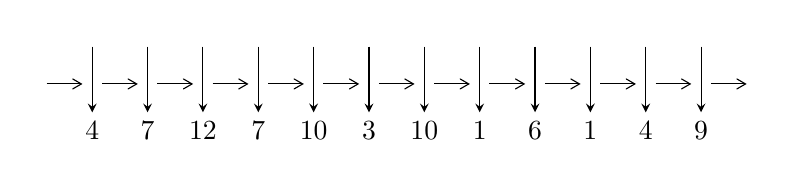
\begin{tikzpicture}[x=20pt, y=17pt]
	% nodes
	\node (C0) at (0, 0) {};
	\node (C1) at (1, 0) {};
	\node (C1U) at (1, +1) {};
	\node (C1D) at (1, -1) {4};

	\node (C2) at (2, 0) {};
	\node (C2U) at (2, +1) {};
	\node (C2D) at (2, -1) {7};

	\node (C3) at (3, 0) {};
	\node (C3U) at (3, +1) {};
	\node (C3D) at (3, -1) {12};

	\node (C4) at (4, 0) {};
	\node (C4U) at (4, +1) {};
	\node (C4D) at (4, -1) {7};

	\node (C5) at (5, 0) {};
	\node (C5U) at (5, +1) {};
	\node (C5D) at (5, -1) {10};

	\node (C6) at (6, 0) {};
	\node (C6U) at (6, +1) {};
	\node (C6D) at (6, -1) {3};

	\node (C7) at (7, 0) {};
	\node (C7U) at (7, +1) {};
	\node (C7D) at (7, -1) {10};

	\node (C8) at (8, 0) {};
	\node (C8U) at (8, +1) {};
	\node (C8D) at (8, -1) {1};

	\node (C9) at (9, 0) {};
	\node (C9U) at (9, +1) {};
	\node (C9D) at (9, -1) {6};

	\node (C10) at (10, 0) {};
	\node (C10U) at (10, +1) {};
	\node (C10D) at (10, -1) {1};

	\node (C11) at (11, 0) {};
	\node (C11U) at (11, +1) {};
	\node (C11D) at (11, -1) {4};

	\node (C12) at (12, 0) {};
	\node (C12U) at (12, +1) {};
	\node (C12D) at (12, -1) {9};
	\node (C13) at (13, 0) {};

	% arrows
	\draw[->,>={angle 60}]
	(C0) edge (C1) (C1) edge (C2) (C2) edge (C3) (C3) edge (C4) (C4) edge (C5) (C5) edge (C6) (C6) edge (C7) (C7) edge (C8) (C8) edge (C9) (C9) edge (C10) (C10) edge (C11) (C11) edge (C12) (C12) edge (C13) ;	\draw[->,>=stealth]
	(C1U) edge (C1D) (C2U) edge (C2D) (C3U) edge (C3D) (C4U) edge (C4D) (C5U) edge (C5D) (C6U) edge (C6D) (C7U) edge (C7D) (C8U) edge (C8D) (C9U) edge (C9D) (C10U) edge (C10D) (C11U) edge (C11D) (C12U) edge (C12D) ;
	\end{tikzpicture} \\
\hhline{~~} \\& 
\textbf{Solving Sequence} \\ \cline{2-2} 
 &
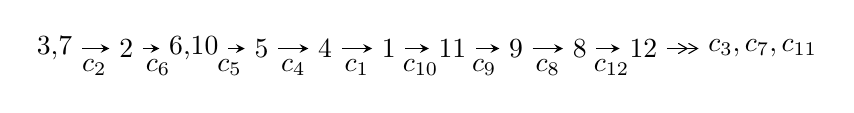
\begin{tikzpicture}[x=23pt, y=7pt]
	% node
	\node (A0) at (-1/8, 0) {3,7};
	\node (A1) at (1, 0) {2};
	\node (A2) at (33/16, 0) {6,10};
	\node (A3) at (25/8, 0) {5};
	\node (A4) at (33/8, 0) {4};
	\node (A5) at (41/8, 0) {1};
	\node (A6) at (49/8, 0) {11};
	\node (A7) at (57/8, 0) {9};
	\node (A8) at (65/8, 0) {8};
	\node (A9) at (73/8, 0) {12};
	\node (C1) at (1/2, -1) {$c_{2}$};
	\node (C2) at (3/2, -1) {$c_{6}$};
	\node (C3) at (21/8, -1) {$c_{5}$};
	\node (C4) at (29/8, -1) {$c_{4}$};
	\node (C5) at (37/8, -1) {$c_{1}$};
	\node (C6) at (45/8, -1) {$c_{10}$};
	\node (C7) at (53/8, -1) {$c_{9}$};
	\node (C8) at (61/8, -1) {$c_{8}$};
	\node (C9) at (69/8, -1) {$c_{12}$};
	\node (A10) at (11, 0) {$c_{3},c_{7},c_{11}$};

	% edge
	\draw[->,>=stealth]	
	(A0) edge (A1) (A1) edge (A2) (A2) edge (A3) (A3) edge (A4) (A4) edge (A5) (A5) edge (A6) (A6) edge (A7) (A7) edge (A8) (A8) edge (A9) ;
	\draw[->>,>={angle 60}]	
	(A9) edge (A10);
\end{tikzpicture} \\ 

\end{tabular} \\

\footnotetext{
The image of knot diagram is generated by the software ``\textbf{Draw programme}" developed by Andrew Bartholomew(\url{http://www.layer8.co.uk/maths/draw/index.htm\#Running-draw}), where we modified some parts for our purpose(\url{https://github.com/CATsTAILs/LinksPainter}).
}\phantom \\ \newline 
\centering \textbf{Ideals for irreducible components\footnotemark of $X_{\text{par}}$} 
 
\begin{align*}
I^u_{1}&=\langle 
u^5- u^4+2 u^3+b+4 u-2,\;u^5- u^4+2 u^3+a+4 u-1,\;u^6-2 u^5+3 u^4-2 u^3+4 u^2-4 u+1\rangle \\
I^u_{2}&=\langle 
- u^5 a- u^4 a-2 u^3 a- a u- u^2+b- u-1,\;- u^5 a-2 u^4 a-4 u^3 a-3 u^2 a+a^2-3 a u+u^2+1,\\
\phantom{I^u_{2}}&\phantom{= \langle  }u^6+u^5+3 u^4+u^3+3 u^2- u+1\rangle \\
I^u_{3}&=\langle 
734 u^{11}-3080 u^{10}+\cdots+7763 b-15155,\;1450 u^{11}-7683 u^{10}+\cdots+7763 a-6462,\\
\phantom{I^u_{3}}&\phantom{= \langle  }u^{12}-5 u^{11}+13 u^{10}-25 u^9+45 u^8-72 u^7+93 u^6-97 u^5+87 u^4-68 u^3+39 u^2-17 u+7\rangle \\
I^u_{4}&=\langle 
- u^7-2 u^4- u^3+u^2+b+1,\;u^9+2 u^6+u^5-2 u^4+a- u,\;u^{10}+u^9+u^7+2 u^6- u^5-3 u^4-2 u^3+u+1\rangle \\
I^u_{5}&=\langle 
- u^9- u^7- u^6- u^5+u^3+2 u^2+b-1,\;- u^9- u^7- u^6- u^5+u^3+2 u^2+a,\\
\phantom{I^u_{5}}&\phantom{= \langle  }u^{10}+u^9+u^7+2 u^6- u^5-3 u^4-2 u^3+u+1\rangle \\
I^u_{6}&=\langle 
u^2+b,\;u^2+a+1,\;u^3- u^2+2 u-1\rangle \\
I^u_{7}&=\langle 
- u^7+5 u^6-12 u^5+19 u^4-20 u^3+14 u^2+b-8 u+3,\\
\phantom{I^u_{7}}&\phantom{= \langle  }-3 u^7+12 u^6-25 u^5+34 u^4-29 u^3+17 u^2+2 a-9 u+2,\\
\phantom{I^u_{7}}&\phantom{= \langle  }u^8-4 u^7+9 u^6-14 u^5+15 u^4-13 u^3+9 u^2-4 u+2\rangle \\
I^u_{8}&=\langle 
a u+u^2+b- a+u+1,\;- u^3 a-2 u^2 a- u^3+a^2- a u- u^2- u,\;u^4+u^3+u^2+1\rangle \\
I^u_{9}&=\langle 
b+1,\;- u^4- u^2+2 a,\;u^6- u^5+u^4+u^3+2\rangle \\
I^u_{10}&=\langle 
b- a-1,\;a^2- a-4,\;u+1\rangle \\
\end{align*}\\
\begin{align*}
I^u_{11}&=\langle 
- u^2+b- u,\;- u^3-3 u^2+a-3 u-2,\;u^4+2 u^3+2 u^2+u-1\rangle \\
I^u_{12}&=\langle 
2 u^3+4 u^2+b+5 u+2,\;2 u^3+4 u^2+a+5 u+3,\;u^4+2 u^3+2 u^2+u-1\rangle \\
\\
\end{align*}
\raggedright * 12 irreducible components of $\dim_{\mathbb{C}}=0$, with total 85 representations.\\
\footnotetext{All coefficients of polynomials are rational numbers. But the coefficients are sometimes approximated in decimal forms when there is not enough margin.}
\newpage
\renewcommand{\arraystretch}{1}
\centering \section*{I. $I^u_{1}= \langle u^5- u^4+2 u^3+b+4 u-2,\;u^5- u^4+2 u^3+a+4 u-1,\;u^6-2 u^5+3 u^4-2 u^3+4 u^2-4 u+1 \rangle$}
\flushleft \textbf{(i) Arc colorings}\\
\begin{tabular}{m{7pt} m{180pt} m{7pt} m{180pt} }
\flushright $a_{3}=$&$\begin{pmatrix}1\\0\end{pmatrix}$ \\
\flushright $a_{7}=$&$\begin{pmatrix}0\\u\end{pmatrix}$ \\
\flushright $a_{2}=$&$\begin{pmatrix}1\\- u^2\end{pmatrix}$ \\
\flushright $a_{6}=$&$\begin{pmatrix}u\\u\end{pmatrix}$ \\
\flushright $a_{10}=$&$\begin{pmatrix}- u^5+u^4-2 u^3-4 u+1\\- u^5+u^4-2 u^3-4 u+2\end{pmatrix}$ \\
\flushright $a_{5}=$&$\begin{pmatrix}u^5- u^4+2 u^3+4 u-1\\u^5- u^4+2 u^3+3 u-1\end{pmatrix}$ \\
\flushright $a_{4}=$&$\begin{pmatrix}u^5- u^4+2 u^3+4 u-1\\u^2\end{pmatrix}$ \\
\flushright $a_{1}=$&$\begin{pmatrix}-3 u^5+4 u^4-6 u^3+2 u^2-11 u+5\\- u^5+u^4- u^3-3 u+1\end{pmatrix}$ \\
\flushright $a_{11}=$&$\begin{pmatrix}3 u^5-4 u^4+7 u^3-2 u^2+11 u-5\\u^3+u\end{pmatrix}$ \\
\flushright $a_{9}=$&$\begin{pmatrix}- u^5+u^4-2 u^3+u^2-4 u+1\\- u^5+u^4-2 u^3+u^2-4 u+2\end{pmatrix}$ \\
\flushright $a_{8}=$&$\begin{pmatrix}-3 u^5+4 u^4-6 u^3+2 u^2-11 u+4\\-2 u^5+3 u^4-4 u^3+2 u^2-7 u+3\end{pmatrix}$ \\
\flushright $a_{12}=$&$\begin{pmatrix}-2 u^5+3 u^4-5 u^3+2 u^2-8 u+4\\- u\end{pmatrix}$\\&\end{tabular}
\flushleft \textbf{(ii) Obstruction class $= -1$}\\~\\
\flushleft \textbf{(iii) Cusp Shapes $= 4 u^5-8 u^4+12 u^3-4 u^2+12 u-20$}\\~\\
\newpage\renewcommand{\arraystretch}{1}
\flushleft \textbf{(iv) u-Polynomials at the component}\newline \\
\begin{tabular}{m{50pt}|m{274pt}}
Crossings & \hspace{64pt}u-Polynomials at each crossing \\
\hline $$\begin{aligned}c_{1},c_{4},c_{7}\\c_{10}\end{aligned}$$&$\begin{aligned}
&u^6-2 u^5-3 u^4+6 u^3+4 u+1
\end{aligned}$\\
\hline $$\begin{aligned}c_{2},c_{3},c_{5}\\c_{6},c_{8},c_{9}\\c_{11},c_{12}\end{aligned}$$&$\begin{aligned}
&u^6+2 u^5+3 u^4+2 u^3+4 u^2+4 u+1
\end{aligned}$\\
\hline
\end{tabular}\\~\\
\newpage\renewcommand{\arraystretch}{1}
\flushleft \textbf{(v) Riley Polynomials at the component}\newline \\
\begin{tabular}{m{50pt}|m{274pt}}
Crossings & \hspace{64pt}Riley Polynomials at each crossing \\
\hline $$\begin{aligned}c_{1},c_{4},c_{7}\\c_{10}\end{aligned}$$&$\begin{aligned}
&y^6-10 y^5+33 y^4-18 y^3-54 y^2-16 y+1
\end{aligned}$\\
\hline $$\begin{aligned}c_{2},c_{3},c_{5}\\c_{6},c_{8},c_{9}\\c_{11},c_{12}\end{aligned}$$&$\begin{aligned}
&y^6+2 y^5+9 y^4+6 y^3+6 y^2-8 y+1
\end{aligned}$\\
\hline
\end{tabular}\\~\\
\newpage\flushleft \textbf{(vi) Complex Volumes and Cusp Shapes}
$$\begin{array}{c|c|c}  
\text{Solutions to }I^u_{1}& \I (\text{vol} + \sqrt{-1}CS) & \text{Cusp shape}\\
 \hline 
\begin{aligned}
u &= -0.565321 + 1.037410 I \\
a &= \phantom{-}0.556120 - 0.294180 I \\
b &= \phantom{-}1.55612 - 0.29418 I\end{aligned}
 & \phantom{-}5.73543 + 5.68242 I & -3.14521 - 5.86849 I \\ \hline\begin{aligned}
u &= -0.565321 - 1.037410 I \\
a &= \phantom{-}0.556120 + 0.294180 I \\
b &= \phantom{-}1.55612 + 0.29418 I\end{aligned}
 & \phantom{-}5.73543 - 5.68242 I & -3.14521 + 5.86849 I \\ \hline\begin{aligned}
u &= \phantom{-}0.716429\phantom{ +0.000000I} \\
a &= -2.52645\phantom{ +0.000000I} \\
b &= -1.52645\phantom{ +0.000000I}\end{aligned}
 & -9.00346\phantom{ +0.000000I} & -10.3960\phantom{ +0.000000I} \\ \hline\begin{aligned}
u &= \phantom{-}0.378183\phantom{ +0.000000I} \\
a &= -0.608191\phantom{ +0.000000I} \\
b &= \phantom{-}0.391809\phantom{ +0.000000I}\end{aligned}
 & -0.650275\phantom{ +0.000000I} & -15.5180\phantom{ +0.000000I} \\ \hline\begin{aligned}
u &= \phantom{-}1.01802 + 1.26802 I \\
a &= \phantom{-}1.011200 - 0.788474 I \\
b &= \phantom{-}2.01120 - 0.78847 I\end{aligned}
 & -8.3108 - 15.2657 I & -11.89809 + 7.17299 I \\ \hline\begin{aligned}
u &= \phantom{-}1.01802 - 1.26802 I \\
a &= \phantom{-}1.011200 + 0.788474 I \\
b &= \phantom{-}2.01120 + 0.78847 I\end{aligned}
 & -8.3108 + 15.2657 I & -11.89809 - 7.17299 I\\
 \hline 
 \end{array}$$\newpage\newpage\renewcommand{\arraystretch}{1}
\centering \section*{II. $I^u_{2}= \langle - u^5 a- u^4 a-2 u^3 a- a u- u^2+b- u-1,\;- u^5 a-2 u^4 a+\cdots+a^2+1,\;u^6+u^5+3 u^4+u^3+3 u^2- u+1 \rangle$}
\flushleft \textbf{(i) Arc colorings}\\
\begin{tabular}{m{7pt} m{180pt} m{7pt} m{180pt} }
\flushright $a_{3}=$&$\begin{pmatrix}1\\0\end{pmatrix}$ \\
\flushright $a_{7}=$&$\begin{pmatrix}0\\u\end{pmatrix}$ \\
\flushright $a_{2}=$&$\begin{pmatrix}1\\- u^2\end{pmatrix}$ \\
\flushright $a_{6}=$&$\begin{pmatrix}u\\u\end{pmatrix}$ \\
\flushright $a_{10}=$&$\begin{pmatrix}a\\u^5 a+u^4 a+2 u^3 a+a u+u^2+u+1\end{pmatrix}$ \\
\flushright $a_{5}=$&$\begin{pmatrix}- a\\- u^5- u^4-2 u^3+a u- u+1\end{pmatrix}$ \\
\flushright $a_{4}=$&$\begin{pmatrix}- a\\- u^5- u^4+u^2 a-2 u^3+a u- u+1\end{pmatrix}$ \\
\flushright $a_{1}=$&$\begin{pmatrix}- u^3- u+1\\- u^4 a+u^5- u^3 a+u^4-2 u^2 a+2 u^3+u^2- a+u-1\end{pmatrix}$ \\
\flushright $a_{11}=$&$\begin{pmatrix}u^4 a+u^5+u^4+u^2 a+2 u^3- a u+a+2 u-1\\u^5 a+2 u^4 a- u^5+2 u^3 a- u^4+2 u^2 a-3 u^3+a u- u^2+a- u+2\end{pmatrix}$ \\
\flushright $a_{9}=$&$\begin{pmatrix}- u^5 a- u^4 a-2 u^3 a+u^4+u^3- a u+u^2+a\\u^4+u^3+2 u^2+u+1\end{pmatrix}$ \\
\flushright $a_{8}=$&$\begin{pmatrix}- u^5 a- u^4 a-2 u^3 a+u^3- a u+a+u\\- u^5 a- u^4 a-2 u^3 a+u^3- a u+u\end{pmatrix}$ \\
\flushright $a_{12}=$&$\begin{pmatrix}- u^4 a- u^5- u^3 a- u^4-2 u^2 a-2 u^3- a- u+1\\- u^4 a- u^3 a-2 u^2 a- a-1\end{pmatrix}$\\&\end{tabular}
\flushleft \textbf{(ii) Obstruction class $= -1$}\\~\\
\flushleft \textbf{(iii) Cusp Shapes $= -3 u^4-7 u^3-10 u^2-9 u-16$}\\~\\
\newpage\renewcommand{\arraystretch}{1}
\flushleft \textbf{(iv) u-Polynomials at the component}\newline \\
\begin{tabular}{m{50pt}|m{274pt}}
Crossings & \hspace{64pt}u-Polynomials at each crossing \\
\hline $$\begin{aligned}c_{1},c_{4},c_{7}\\c_{10}\end{aligned}$$&$\begin{aligned}
&u^{12}- u^{11}+\cdots-11 u+1
\end{aligned}$\\
\hline $$\begin{aligned}c_{2},c_{6},c_{8}\\c_{12}\end{aligned}$$&$\begin{aligned}
&(u^6- u^5+3 u^4- u^3+3 u^2+u+1)^2
\end{aligned}$\\
\hline $$\begin{aligned}c_{3},c_{5},c_{9}\\c_{11}\end{aligned}$$&$\begin{aligned}
&u^{12}+5 u^{11}+\cdots+17 u+7
\end{aligned}$\\
\hline
\end{tabular}\\~\\
\newpage\renewcommand{\arraystretch}{1}
\flushleft \textbf{(v) Riley Polynomials at the component}\newline \\
\begin{tabular}{m{50pt}|m{274pt}}
Crossings & \hspace{64pt}Riley Polynomials at each crossing \\
\hline $$\begin{aligned}c_{1},c_{4},c_{7}\\c_{10}\end{aligned}$$&$\begin{aligned}
&y^{12}-19 y^{11}+\cdots-37 y+1
\end{aligned}$\\
\hline $$\begin{aligned}c_{2},c_{6},c_{8}\\c_{12}\end{aligned}$$&$\begin{aligned}
&(y^6+5 y^5+13 y^4+21 y^3+17 y^2+5 y+1)^2
\end{aligned}$\\
\hline $$\begin{aligned}c_{3},c_{5},c_{9}\\c_{11}\end{aligned}$$&$\begin{aligned}
&y^{12}+y^{11}+\cdots+257 y+49
\end{aligned}$\\
\hline
\end{tabular}\\~\\
\newpage\flushleft \textbf{(vi) Complex Volumes and Cusp Shapes}
$$\begin{array}{c|c|c}  
\text{Solutions to }I^u_{2}& \I (\text{vol} + \sqrt{-1}CS) & \text{Cusp shape}\\
 \hline 
\begin{aligned}
u &= \phantom{-}0.028955 + 1.263070 I \\
a &= \phantom{-}0.565560 - 0.864727 I \\
b &= \phantom{-}1.113440 - 0.846070 I\end{aligned}
 & \phantom{-}4.88968 - 2.84039 I & -6.95695 + 2.68362 I \\ \hline\begin{aligned}
u &= \phantom{-}0.028955 + 1.263070 I \\
a &= -0.374177 - 0.442775 I \\
b &= -1.46946 + 0.08347 I\end{aligned}
 & \phantom{-}4.88968 - 2.84039 I & -6.95695 + 2.68362 I \\ \hline\begin{aligned}
u &= \phantom{-}0.028955 - 1.263070 I \\
a &= \phantom{-}0.565560 + 0.864727 I \\
b &= \phantom{-}1.113440 + 0.846070 I\end{aligned}
 & \phantom{-}4.88968 + 2.84039 I & -6.95695 - 2.68362 I \\ \hline\begin{aligned}
u &= \phantom{-}0.028955 - 1.263070 I \\
a &= -0.374177 + 0.442775 I \\
b &= -1.46946 - 0.08347 I\end{aligned}
 & \phantom{-}4.88968 + 2.84039 I & -6.95695 - 2.68362 I \\ \hline\begin{aligned}
u &= -0.80039 + 1.17645 I \\
a &= -1.035600 - 0.905749 I \\
b &= -1.97804 - 1.00830 I\end{aligned}
 & -9.60039 + 6.66133 I & -12.05452 - 4.58491 I \\ \hline\begin{aligned}
u &= -0.80039 + 1.17645 I \\
a &= \phantom{-}0.760760 + 1.153110 I \\
b &= \phantom{-}0.764071 - 0.032173 I\end{aligned}
 & -9.60039 + 6.66133 I & -12.05452 - 4.58491 I \\ \hline\begin{aligned}
u &= -0.80039 - 1.17645 I \\
a &= -1.035600 + 0.905749 I \\
b &= -1.97804 + 1.00830 I\end{aligned}
 & -9.60039 - 6.66133 I & -12.05452 + 4.58491 I \\ \hline\begin{aligned}
u &= -0.80039 - 1.17645 I \\
a &= \phantom{-}0.760760 - 1.153110 I \\
b &= \phantom{-}0.764071 + 0.032173 I\end{aligned}
 & -9.60039 - 6.66133 I & -12.05452 + 4.58491 I \\ \hline\begin{aligned}
u &= \phantom{-}0.271430 + 0.485552 I \\
a &= \phantom{-}0.041323 - 0.362162 I \\
b &= \phantom{-}1.22951 + 0.79439 I\end{aligned}
 & -1.04656 + 1.35140 I & -15.4885 - 6.6994 I \\ \hline\begin{aligned}
u &= \phantom{-}0.271430 + 0.485552 I \\
a &= -0.45786 + 2.36589 I \\
b &= \phantom{-}0.340472 + 0.389317 I\end{aligned}
 & -1.04656 + 1.35140 I & -15.4885 - 6.6994 I\\
 \hline 
 \end{array}$$\newpage$$\begin{array}{c|c|c}  
\text{Solutions to }I^u_{2}& \I (\text{vol} + \sqrt{-1}CS) & \text{Cusp shape}\\
 \hline 
\begin{aligned}
u &= \phantom{-}0.271430 - 0.485552 I \\
a &= \phantom{-}0.041323 + 0.362162 I \\
b &= \phantom{-}1.22951 - 0.79439 I\end{aligned}
 & -1.04656 - 1.35140 I & -15.4885 + 6.6994 I \\ \hline\begin{aligned}
u &= \phantom{-}0.271430 - 0.485552 I \\
a &= -0.45786 - 2.36589 I \\
b &= \phantom{-}0.340472 - 0.389317 I\end{aligned}
 & -1.04656 - 1.35140 I & -15.4885 + 6.6994 I\\
 \hline 
 \end{array}$$\newpage\newpage\renewcommand{\arraystretch}{1}
\centering \section*{III. $I^u_{3}= \langle 734 u^{11}-3080 u^{10}+\cdots+7763 b-15155,\;1450 u^{11}-7683 u^{10}+\cdots+7763 a-6462,\;u^{12}-5 u^{11}+\cdots-17 u+7 \rangle$}
\flushleft \textbf{(i) Arc colorings}\\
\begin{tabular}{m{7pt} m{180pt} m{7pt} m{180pt} }
\flushright $a_{3}=$&$\begin{pmatrix}1\\0\end{pmatrix}$ \\
\flushright $a_{7}=$&$\begin{pmatrix}0\\u\end{pmatrix}$ \\
\flushright $a_{2}=$&$\begin{pmatrix}1\\- u^2\end{pmatrix}$ \\
\flushright $a_{6}=$&$\begin{pmatrix}u\\u\end{pmatrix}$ \\
\flushright $a_{10}=$&$\begin{pmatrix}-0.186783 u^{11}+0.989695 u^{10}+\cdots-4.53265 u+0.832410\\-0.0945511 u^{11}+0.396754 u^{10}+\cdots-3.56421 u+1.95221\end{pmatrix}$ \\
\flushright $a_{5}=$&$\begin{pmatrix}-0.147108 u^{11}+0.473657 u^{10}+\cdots+4.45537 u-2.03465\\-0.261883 u^{11}+1.26240 u^{10}+\cdots-4.53549 u+1.02976\end{pmatrix}$ \\
\flushright $a_{4}=$&$\begin{pmatrix}-0.147108 u^{11}+0.473657 u^{10}+\cdots+4.45537 u-2.03465\\-0.214865 u^{11}+0.915239 u^{10}+\cdots-1.11323 u-0.803427\end{pmatrix}$ \\
\flushright $a_{1}=$&$\begin{pmatrix}-0.267809 u^{11}+0.983254 u^{10}+\cdots+2.83086 u-1.89733\\-0.107948 u^{11}+0.660054 u^{10}+\cdots-3.27631 u-0.615870\end{pmatrix}$ \\
\flushright $a_{11}=$&$\begin{pmatrix}-0.0769033 u^{11}+0.516939 u^{10}+\cdots-1.73606 u+0.269226\\-0.154322 u^{11}+0.879170 u^{10}+\cdots-5.04895 u+2.11001\end{pmatrix}$ \\
\flushright $a_{9}=$&$\begin{pmatrix}-0.448023 u^{11}+2.12405 u^{10}+\cdots-7.41852 u+1.75486\\-0.355790 u^{11}+1.53111 u^{10}+\cdots-6.45008 u+2.87466\end{pmatrix}$ \\
\flushright $a_{8}=$&$\begin{pmatrix}0.0617029 u^{11}-0.295118 u^{10}+\cdots+1.00502 u-0.336854\\-0.0854051 u^{11}+0.178539 u^{10}+\cdots+5.46039 u-2.37151\end{pmatrix}$ \\
\flushright $a_{12}=$&$\begin{pmatrix}-0.278887 u^{11}+1.29988 u^{10}+\cdots-5.42831 u+1.17686\\0.131779 u^{11}-0.397656 u^{10}+\cdots-2.68775 u+0.645627\end{pmatrix}$\\&\end{tabular}
\flushleft \textbf{(ii) Obstruction class $= -1$}\\~\\
\flushleft \textbf{(iii) Cusp Shapes $= \frac{21796}{7763} u^{11}-\frac{13936}{1109} u^{10}+\frac{237890}{7763} u^9-\frac{434843}{7763} u^8+\frac{110031}{1109} u^7-\frac{1172937}{7763} u^6+\frac{1426749}{7763} u^5-\frac{1359518}{7763} u^4+\frac{1096584}{7763} u^3-\frac{724103}{7763} u^2+\frac{299834}{7763} u-\frac{28345}{1109}$}\\~\\
\newpage\renewcommand{\arraystretch}{1}
\flushleft \textbf{(iv) u-Polynomials at the component}\newline \\
\begin{tabular}{m{50pt}|m{274pt}}
Crossings & \hspace{64pt}u-Polynomials at each crossing \\
\hline $$\begin{aligned}c_{1},c_{4},c_{7}\\c_{10}\end{aligned}$$&$\begin{aligned}
&u^{12}- u^{11}+\cdots-11 u+1
\end{aligned}$\\
\hline $$\begin{aligned}c_{2},c_{6},c_{8}\\c_{12}\end{aligned}$$&$\begin{aligned}
&u^{12}+5 u^{11}+\cdots+17 u+7
\end{aligned}$\\
\hline $$\begin{aligned}c_{3},c_{5},c_{9}\\c_{11}\end{aligned}$$&$\begin{aligned}
&(u^6- u^5+3 u^4- u^3+3 u^2+u+1)^2
\end{aligned}$\\
\hline
\end{tabular}\\~\\
\newpage\renewcommand{\arraystretch}{1}
\flushleft \textbf{(v) Riley Polynomials at the component}\newline \\
\begin{tabular}{m{50pt}|m{274pt}}
Crossings & \hspace{64pt}Riley Polynomials at each crossing \\
\hline $$\begin{aligned}c_{1},c_{4},c_{7}\\c_{10}\end{aligned}$$&$\begin{aligned}
&y^{12}-19 y^{11}+\cdots-37 y+1
\end{aligned}$\\
\hline $$\begin{aligned}c_{2},c_{6},c_{8}\\c_{12}\end{aligned}$$&$\begin{aligned}
&y^{12}+y^{11}+\cdots+257 y+49
\end{aligned}$\\
\hline $$\begin{aligned}c_{3},c_{5},c_{9}\\c_{11}\end{aligned}$$&$\begin{aligned}
&(y^6+5 y^5+13 y^4+21 y^3+17 y^2+5 y+1)^2
\end{aligned}$\\
\hline
\end{tabular}\\~\\
\newpage\flushleft \textbf{(vi) Complex Volumes and Cusp Shapes}
$$\begin{array}{c|c|c}  
\text{Solutions to }I^u_{3}& \I (\text{vol} + \sqrt{-1}CS) & \text{Cusp shape}\\
 \hline 
\begin{aligned}
u &= -0.239056 + 0.890852 I \\
a &= \phantom{-}0.79735 + 1.21505 I \\
b &= \phantom{-}1.22951 + 0.79439 I\end{aligned}
 & -1.04656 + 1.35140 I & -15.4885 - 6.6994 I \\ \hline\begin{aligned}
u &= -0.239056 - 0.890852 I \\
a &= \phantom{-}0.79735 - 1.21505 I \\
b &= \phantom{-}1.22951 - 0.79439 I\end{aligned}
 & -1.04656 - 1.35140 I & -15.4885 + 6.6994 I \\ \hline\begin{aligned}
u &= \phantom{-}1.176420 + 0.148869 I \\
a &= \phantom{-}0.164789 + 0.045651 I \\
b &= \phantom{-}0.340472 - 0.389317 I\end{aligned}
 & -1.04656 - 1.35140 I & -15.4885 + 6.6994 I \\ \hline\begin{aligned}
u &= \phantom{-}1.176420 - 0.148869 I \\
a &= \phantom{-}0.164789 - 0.045651 I \\
b &= \phantom{-}0.340472 + 0.389317 I\end{aligned}
 & -1.04656 + 1.35140 I & -15.4885 - 6.6994 I \\ \hline\begin{aligned}
u &= -0.007700 + 0.692554 I \\
a &= -0.709646 - 0.783990 I \\
b &= \phantom{-}1.113440 - 0.846070 I\end{aligned}
 & \phantom{-}4.88968 - 2.84039 I & -6.95695 + 2.68362 I \\ \hline\begin{aligned}
u &= -0.007700 - 0.692554 I \\
a &= -0.709646 + 0.783990 I \\
b &= \phantom{-}1.113440 + 0.846070 I\end{aligned}
 & \phantom{-}4.88968 + 2.84039 I & -6.95695 - 2.68362 I \\ \hline\begin{aligned}
u &= \phantom{-}0.874959 + 1.026640 I \\
a &= -0.92937 + 1.12242 I \\
b &= -1.97804 + 1.00830 I\end{aligned}
 & -9.60039 - 6.66133 I & -12.05452 + 4.58491 I \\ \hline\begin{aligned}
u &= \phantom{-}0.874959 - 1.026640 I \\
a &= -0.92937 - 1.12242 I \\
b &= -1.97804 - 1.00830 I\end{aligned}
 & -9.60039 + 6.66133 I & -12.05452 - 4.58491 I \\ \hline\begin{aligned}
u &= -0.69640 + 1.36818 I \\
a &= -0.727697 - 0.439865 I \\
b &= -1.46946 - 0.08347 I\end{aligned}
 & \phantom{-}4.88968 + 2.84039 I & -6.95695 - 2.68362 I \\ \hline\begin{aligned}
u &= -0.69640 - 1.36818 I \\
a &= -0.727697 + 0.439865 I \\
b &= -1.46946 + 0.08347 I\end{aligned}
 & \phantom{-}4.88968 - 2.84039 I & -6.95695 + 2.68362 I\\
 \hline 
 \end{array}$$\newpage$$\begin{array}{c|c|c}  
\text{Solutions to }I^u_{3}& \I (\text{vol} + \sqrt{-1}CS) & \text{Cusp shape}\\
 \hline 
\begin{aligned}
u &= \phantom{-}1.39178 + 0.95258 I \\
a &= \phantom{-}0.761714 - 0.875845 I \\
b &= \phantom{-}0.764071 - 0.032173 I\end{aligned}
 & -9.60039 + 6.66133 I & -12.05452 - 4.58491 I \\ \hline\begin{aligned}
u &= \phantom{-}1.39178 - 0.95258 I \\
a &= \phantom{-}0.761714 + 0.875845 I \\
b &= \phantom{-}0.764071 + 0.032173 I\end{aligned}
 & -9.60039 - 6.66133 I & -12.05452 + 4.58491 I\\
 \hline 
 \end{array}$$\newpage\newpage\renewcommand{\arraystretch}{1}
\centering \section*{IV. $I^u_{4}= \langle - u^7-2 u^4- u^3+u^2+b+1,\;u^9+2 u^6+u^5-2 u^4+a- u,\;u^{10}+u^9+u^7+2 u^6- u^5-3 u^4-2 u^3+u+1 \rangle$}
\flushleft \textbf{(i) Arc colorings}\\
\begin{tabular}{m{7pt} m{180pt} m{7pt} m{180pt} }
\flushright $a_{3}=$&$\begin{pmatrix}1\\0\end{pmatrix}$ \\
\flushright $a_{7}=$&$\begin{pmatrix}0\\u\end{pmatrix}$ \\
\flushright $a_{2}=$&$\begin{pmatrix}1\\- u^2\end{pmatrix}$ \\
\flushright $a_{6}=$&$\begin{pmatrix}u\\u\end{pmatrix}$ \\
\flushright $a_{10}=$&$\begin{pmatrix}- u^9-2 u^6- u^5+2 u^4+u\\u^7+2 u^4+u^3- u^2-1\end{pmatrix}$ \\
\flushright $a_{5}=$&$\begin{pmatrix}- u^9- u^7- u^6- u^5+u^3+2 u^2\\-2 u^9-3 u^6- u^5+3 u^4+2 u^3+2 u^2-1\end{pmatrix}$ \\
\flushright $a_{4}=$&$\begin{pmatrix}- u^9- u^7- u^6- u^5+u^3+2 u^2\\u^2\end{pmatrix}$ \\
\flushright $a_{1}=$&$\begin{pmatrix}u^8+u^6+u^5+u^4- u^2- u\\2 u^9+u^8- u^7+3 u^6+2 u^5-4 u^4-4 u^3-2 u^2+2\end{pmatrix}$ \\
\flushright $a_{11}=$&$\begin{pmatrix}2 u^9- u^8+u^6-4 u^4-3 u^3- u^2+3 u+2\\u^3+u\end{pmatrix}$ \\
\flushright $a_{9}=$&$\begin{pmatrix}u^9+u^8+u^6+2 u^5-3 u^3-2 u^2+u+1\\2 u^9+u^8+u^7+3 u^6+3 u^5-2 u^3-3 u^2\end{pmatrix}$ \\
\flushright $a_{8}=$&$\begin{pmatrix}2 u^9+u^8+2 u^6+3 u^5-2 u^4-4 u^3-3 u^2+u+2\\u^9+u^8- u^7+u^6+2 u^5-2 u^4-3 u^3- u^2+u+2\end{pmatrix}$ \\
\flushright $a_{12}=$&$\begin{pmatrix}- u^9- u^5+2 u^4+3 u^3+u^2-2 u-1\\- u\end{pmatrix}$\\&\end{tabular}
\flushleft \textbf{(ii) Obstruction class $= -1$}\\~\\
\flushleft \textbf{(iii) Cusp Shapes $= -13 u^9-9 u^8-2 u^7-20 u^6-24 u^5+8 u^4+21 u^3+16 u^2+2 u-18$}\\~\\
\newpage\renewcommand{\arraystretch}{1}
\flushleft \textbf{(iv) u-Polynomials at the component}\newline \\
\begin{tabular}{m{50pt}|m{274pt}}
Crossings & \hspace{64pt}u-Polynomials at each crossing \\
\hline $$\begin{aligned}c_{1},c_{7}\end{aligned}$$&$\begin{aligned}
&u^{10}-2 u^9-2 u^8+12 u^6+9 u^5-43 u^4+11 u^3+37 u^2-29 u+7
\end{aligned}$\\
\hline $$\begin{aligned}c_{2},c_{3},c_{5}\\c_{6},c_{8},c_{9}\\c_{11},c_{12}\end{aligned}$$&$\begin{aligned}
&u^{10}- u^9- u^7+2 u^6+u^5-3 u^4+2 u^3- u+1
\end{aligned}$\\
\hline $$\begin{aligned}c_{4},c_{10}\end{aligned}$$&$\begin{aligned}
&(u^5+2 u^4-2 u^3-2 u^2+u+1)^2
\end{aligned}$\\
\hline
\end{tabular}\\~\\
\newpage\renewcommand{\arraystretch}{1}
\flushleft \textbf{(v) Riley Polynomials at the component}\newline \\
\begin{tabular}{m{50pt}|m{274pt}}
Crossings & \hspace{64pt}Riley Polynomials at each crossing \\
\hline $$\begin{aligned}c_{1},c_{7}\end{aligned}$$&$\begin{aligned}
&y^{10}-8 y^9+\cdots-323 y+49
\end{aligned}$\\
\hline $$\begin{aligned}c_{2},c_{3},c_{5}\\c_{6},c_{8},c_{9}\\c_{11},c_{12}\end{aligned}$$&$\begin{aligned}
&y^{10}- y^9+2 y^8-5 y^7+10 y^6-9 y^5+3 y^4+2 y^3-2 y^2- y+1
\end{aligned}$\\
\hline $$\begin{aligned}c_{4},c_{10}\end{aligned}$$&$\begin{aligned}
&(y^5-8 y^4+14 y^3-12 y^2+5 y-1)^2
\end{aligned}$\\
\hline
\end{tabular}\\~\\
\newpage\flushleft \textbf{(vi) Complex Volumes and Cusp Shapes}
$$\begin{array}{c|c|c}  
\text{Solutions to }I^u_{4}& \I (\text{vol} + \sqrt{-1}CS) & \text{Cusp shape}\\
 \hline 
\begin{aligned}
u &= -0.833438 + 0.554152 I \\
a &= -0.812076 - 0.979588 I \\
b &= -2.03262 - 0.35101 I\end{aligned}
 & \phantom{-}1.24137 + 6.64784 I & -13.9589 - 7.4975 I \\ \hline\begin{aligned}
u &= -0.833438 - 0.554152 I \\
a &= -0.812076 + 0.979588 I \\
b &= -2.03262 + 0.35101 I\end{aligned}
 & \phantom{-}1.24137 - 6.64784 I & -13.9589 + 7.4975 I \\ \hline\begin{aligned}
u &= -1.016860 + 0.408978 I \\
a &= -1.31220 - 0.69239 I \\
b &= -0.590675\phantom{ +0.000000I}\end{aligned}
 & -11.5552\phantom{ +0.000000I} & -19.8669 + 0. I\phantom{ +0.000000I} \\ \hline\begin{aligned}
u &= -1.016860 - 0.408978 I \\
a &= -1.31220 + 0.69239 I \\
b &= -0.590675\phantom{ +0.000000I}\end{aligned}
 & -11.5552\phantom{ +0.000000I} & -19.8669 + 0. I\phantom{ +0.000000I} \\ \hline\begin{aligned}
u &= \phantom{-}0.868230 + 0.062281 I \\
a &= \phantom{-}0.481330 - 0.323224 I \\
b &= \phantom{-}0.327959 + 0.538837 I\end{aligned}
 & -1.22103 + 1.14013 I & -11.60766 - 5.93486 I \\ \hline\begin{aligned}
u &= \phantom{-}0.868230 - 0.062281 I \\
a &= \phantom{-}0.481330 + 0.323224 I \\
b &= \phantom{-}0.327959 - 0.538837 I\end{aligned}
 & -1.22103 - 1.14013 I & -11.60766 + 5.93486 I \\ \hline\begin{aligned}
u &= -0.186852 + 0.738915 I \\
a &= \phantom{-}0.52801 + 1.66326 I \\
b &= \phantom{-}0.327959 + 0.538837 I\end{aligned}
 & -1.22103 + 1.14013 I & -11.60766 - 5.93486 I \\ \hline\begin{aligned}
u &= -0.186852 - 0.738915 I \\
a &= \phantom{-}0.52801 - 1.66326 I \\
b &= \phantom{-}0.327959 - 0.538837 I\end{aligned}
 & -1.22103 - 1.14013 I & -11.60766 + 5.93486 I \\ \hline\begin{aligned}
u &= \phantom{-}0.668920 + 1.200250 I \\
a &= -1.385060 + 0.017518 I \\
b &= -2.03262 + 0.35101 I\end{aligned}
 & \phantom{-}1.24137 - 6.64784 I & -13.9589 + 7.4975 I \\ \hline\begin{aligned}
u &= \phantom{-}0.668920 - 1.200250 I \\
a &= -1.385060 - 0.017518 I \\
b &= -2.03262 - 0.35101 I\end{aligned}
 & \phantom{-}1.24137 + 6.64784 I & -13.9589 - 7.4975 I\\
 \hline 
 \end{array}$$\newpage\newpage\renewcommand{\arraystretch}{1}
\centering \section*{V. $I^u_{5}= \langle - u^9- u^7- u^6- u^5+u^3+2 u^2+b-1,\;- u^9- u^7- u^6- u^5+u^3+2 u^2+a,\;u^{10}+u^9+u^7+2 u^6- u^5-3 u^4-2 u^3+u+1 \rangle$}
\flushleft \textbf{(i) Arc colorings}\\
\begin{tabular}{m{7pt} m{180pt} m{7pt} m{180pt} }
\flushright $a_{3}=$&$\begin{pmatrix}1\\0\end{pmatrix}$ \\
\flushright $a_{7}=$&$\begin{pmatrix}0\\u\end{pmatrix}$ \\
\flushright $a_{2}=$&$\begin{pmatrix}1\\- u^2\end{pmatrix}$ \\
\flushright $a_{6}=$&$\begin{pmatrix}u\\u\end{pmatrix}$ \\
\flushright $a_{10}=$&$\begin{pmatrix}u^9+u^7+u^6+u^5- u^3-2 u^2\\u^9+u^7+u^6+u^5- u^3-2 u^2+1\end{pmatrix}$ \\
\flushright $a_{5}=$&$\begin{pmatrix}u^9- u^8+u^6- u^5-2 u^4+2 u+1\\u^9- u^8+u^6- u^5-2 u^4+u+1\end{pmatrix}$ \\
\flushright $a_{4}=$&$\begin{pmatrix}u^9- u^8+u^6- u^5-2 u^4+2 u+1\\- u^9- u^8+u^7-2 u^6-2 u^5+2 u^4+2 u^3-1\end{pmatrix}$ \\
\flushright $a_{1}=$&$\begin{pmatrix}u^8+u^6+u^5+u^4- u^2- u\\- u^9- u^6- u^5+2 u^4+u^3-1\end{pmatrix}$ \\
\flushright $a_{11}=$&$\begin{pmatrix}u^9+u^8+2 u^6+2 u^5-2 u^3-2 u^2\\- u^9+u^7- u^6- u^5+4 u^4+2 u^3- u^2- u-1\end{pmatrix}$ \\
\flushright $a_{9}=$&$\begin{pmatrix}u^9+u^7+u^6+u^5- u^3- u^2\\u^9+u^7+u^6+u^5- u^3- u^2+1\end{pmatrix}$ \\
\flushright $a_{8}=$&$\begin{pmatrix}2 u^9+u^7+2 u^6+2 u^5-2 u^4-2 u^3-2 u^2+1\\3 u^9- u^8+u^7+3 u^6+u^5-4 u^4-2 u^3-2 u^2+2 u+2\end{pmatrix}$ \\
\flushright $a_{12}=$&$\begin{pmatrix}u^9+u^8+2 u^6+2 u^5- u^4- u^3- u^2- u+1\\u^9- u^8- u^7+u^6- u^5-4 u^4- u^3+u^2+2 u+1\end{pmatrix}$\\&\end{tabular}
\flushleft \textbf{(ii) Obstruction class $= -1$}\\~\\
\flushleft \textbf{(iii) Cusp Shapes $= -13 u^9-9 u^8-2 u^7-20 u^6-24 u^5+8 u^4+21 u^3+16 u^2+2 u-18$}\\~\\
\newpage\renewcommand{\arraystretch}{1}
\flushleft \textbf{(iv) u-Polynomials at the component}\newline \\
\begin{tabular}{m{50pt}|m{274pt}}
Crossings & \hspace{64pt}u-Polynomials at each crossing \\
\hline $$\begin{aligned}c_{1},c_{7}\end{aligned}$$&$\begin{aligned}
&(u^5+2 u^4-2 u^3-2 u^2+u+1)^2
\end{aligned}$\\
\hline $$\begin{aligned}c_{2},c_{3},c_{5}\\c_{6},c_{8},c_{9}\\c_{11},c_{12}\end{aligned}$$&$\begin{aligned}
&u^{10}- u^9- u^7+2 u^6+u^5-3 u^4+2 u^3- u+1
\end{aligned}$\\
\hline $$\begin{aligned}c_{4},c_{10}\end{aligned}$$&$\begin{aligned}
&u^{10}-2 u^9-2 u^8+12 u^6+9 u^5-43 u^4+11 u^3+37 u^2-29 u+7
\end{aligned}$\\
\hline
\end{tabular}\\~\\
\newpage\renewcommand{\arraystretch}{1}
\flushleft \textbf{(v) Riley Polynomials at the component}\newline \\
\begin{tabular}{m{50pt}|m{274pt}}
Crossings & \hspace{64pt}Riley Polynomials at each crossing \\
\hline $$\begin{aligned}c_{1},c_{7}\end{aligned}$$&$\begin{aligned}
&(y^5-8 y^4+14 y^3-12 y^2+5 y-1)^2
\end{aligned}$\\
\hline $$\begin{aligned}c_{2},c_{3},c_{5}\\c_{6},c_{8},c_{9}\\c_{11},c_{12}\end{aligned}$$&$\begin{aligned}
&y^{10}- y^9+2 y^8-5 y^7+10 y^6-9 y^5+3 y^4+2 y^3-2 y^2- y+1
\end{aligned}$\\
\hline $$\begin{aligned}c_{4},c_{10}\end{aligned}$$&$\begin{aligned}
&y^{10}-8 y^9+\cdots-323 y+49
\end{aligned}$\\
\hline
\end{tabular}\\~\\
\newpage\flushleft \textbf{(vi) Complex Volumes and Cusp Shapes}
$$\begin{array}{c|c|c}  
\text{Solutions to }I^u_{5}& \I (\text{vol} + \sqrt{-1}CS) & \text{Cusp shape}\\
 \hline 
\begin{aligned}
u &= -0.833438 + 0.554152 I \\
a &= -0.885525 - 0.234725 I \\
b &= \phantom{-}0.114475 - 0.234725 I\end{aligned}
 & \phantom{-}1.24137 + 6.64784 I & -13.9589 - 7.4975 I \\ \hline\begin{aligned}
u &= -0.833438 - 0.554152 I \\
a &= -0.885525 + 0.234725 I \\
b &= \phantom{-}0.114475 + 0.234725 I\end{aligned}
 & \phantom{-}1.24137 - 6.64784 I & -13.9589 + 7.4975 I \\ \hline\begin{aligned}
u &= -1.016860 + 0.408978 I \\
a &= \phantom{-}2.06801 + 0.83175 I \\
b &= \phantom{-}3.06801 + 0.83175 I\end{aligned}
 & -11.5552\phantom{ +0.000000I} & -19.8669 + 0. I\phantom{ +0.000000I} \\ \hline\begin{aligned}
u &= -1.016860 - 0.408978 I \\
a &= \phantom{-}2.06801 - 0.83175 I \\
b &= \phantom{-}3.06801 - 0.83175 I\end{aligned}
 & -11.5552\phantom{ +0.000000I} & -19.8669 + 0. I\phantom{ +0.000000I} \\ \hline\begin{aligned}
u &= \phantom{-}0.868230 + 0.062281 I \\
a &= -0.719333 + 0.353776 I \\
b &= \phantom{-}0.280667 + 0.353776 I\end{aligned}
 & -1.22103 + 1.14013 I & -11.60766 - 5.93486 I \\ \hline\begin{aligned}
u &= \phantom{-}0.868230 - 0.062281 I \\
a &= -0.719333 - 0.353776 I \\
b &= \phantom{-}0.280667 - 0.353776 I\end{aligned}
 & -1.22103 - 1.14013 I & -11.60766 + 5.93486 I \\ \hline\begin{aligned}
u &= -0.186852 + 0.738915 I \\
a &= \phantom{-}0.541694 + 0.738059 I \\
b &= \phantom{-}1.54169 + 0.73806 I\end{aligned}
 & -1.22103 + 1.14013 I & -11.60766 - 5.93486 I \\ \hline\begin{aligned}
u &= -0.186852 - 0.738915 I \\
a &= \phantom{-}0.541694 - 0.738059 I \\
b &= \phantom{-}1.54169 - 0.73806 I\end{aligned}
 & -1.22103 - 1.14013 I & -11.60766 + 5.93486 I \\ \hline\begin{aligned}
u &= \phantom{-}0.668920 + 1.200250 I \\
a &= \phantom{-}0.495151 - 0.447313 I \\
b &= \phantom{-}1.49515 - 0.44731 I\end{aligned}
 & \phantom{-}1.24137 - 6.64784 I & -13.9589 + 7.4975 I \\ \hline\begin{aligned}
u &= \phantom{-}0.668920 - 1.200250 I \\
a &= \phantom{-}0.495151 + 0.447313 I \\
b &= \phantom{-}1.49515 + 0.44731 I\end{aligned}
 & \phantom{-}1.24137 + 6.64784 I & -13.9589 - 7.4975 I\\
 \hline 
 \end{array}$$\newpage\newpage\renewcommand{\arraystretch}{1}
\centering \section*{VI. $I^u_{6}= \langle u^2+b,\;u^2+a+1,\;u^3- u^2+2 u-1 \rangle$}
\flushleft \textbf{(i) Arc colorings}\\
\begin{tabular}{m{7pt} m{180pt} m{7pt} m{180pt} }
\flushright $a_{3}=$&$\begin{pmatrix}1\\0\end{pmatrix}$ \\
\flushright $a_{7}=$&$\begin{pmatrix}0\\u\end{pmatrix}$ \\
\flushright $a_{2}=$&$\begin{pmatrix}1\\- u^2\end{pmatrix}$ \\
\flushright $a_{6}=$&$\begin{pmatrix}u\\u\end{pmatrix}$ \\
\flushright $a_{10}=$&$\begin{pmatrix}- u^2-1\\- u^2\end{pmatrix}$ \\
\flushright $a_{5}=$&$\begin{pmatrix}u^2+1\\u^2- u+1\end{pmatrix}$ \\
\flushright $a_{4}=$&$\begin{pmatrix}u^2+1\\u^2\end{pmatrix}$ \\
\flushright $a_{1}=$&$\begin{pmatrix}0\\- u\end{pmatrix}$ \\
\flushright $a_{11}=$&$\begin{pmatrix}- u^2-1\\- u^2+u-1\end{pmatrix}$ \\
\flushright $a_{9}=$&$\begin{pmatrix}-1\\0\end{pmatrix}$ \\
\flushright $a_{8}=$&$\begin{pmatrix}-1\\u^2\end{pmatrix}$ \\
\flushright $a_{12}=$&$\begin{pmatrix}- u\\- u\end{pmatrix}$\\&\end{tabular}
\flushleft \textbf{(ii) Obstruction class $= 1$}\\~\\
\flushleft \textbf{(iii) Cusp Shapes $= -8 u^2+8 u-20$}\\~\\
\newpage\renewcommand{\arraystretch}{1}
\flushleft \textbf{(iv) u-Polynomials at the component}\newline \\
\begin{tabular}{m{50pt}|m{274pt}}
Crossings & \hspace{64pt}u-Polynomials at each crossing \\
\hline $$\begin{aligned}c_{1},c_{4},c_{7}\\c_{10}\end{aligned}$$&$\begin{aligned}
&u^3+u^2-1
\end{aligned}$\\
\hline $$\begin{aligned}c_{2},c_{5},c_{8}\\c_{11}\end{aligned}$$&$\begin{aligned}
&u^3- u^2+2 u-1
\end{aligned}$\\
\hline $$\begin{aligned}c_{3},c_{6},c_{9}\\c_{12}\end{aligned}$$&$\begin{aligned}
&u^3+u^2+2 u+1
\end{aligned}$\\
\hline
\end{tabular}\\~\\
\newpage\renewcommand{\arraystretch}{1}
\flushleft \textbf{(v) Riley Polynomials at the component}\newline \\
\begin{tabular}{m{50pt}|m{274pt}}
Crossings & \hspace{64pt}Riley Polynomials at each crossing \\
\hline $$\begin{aligned}c_{1},c_{4},c_{7}\\c_{10}\end{aligned}$$&$\begin{aligned}
&y^3- y^2+2 y-1
\end{aligned}$\\
\hline $$\begin{aligned}c_{2},c_{3},c_{5}\\c_{6},c_{8},c_{9}\\c_{11},c_{12}\end{aligned}$$&$\begin{aligned}
&y^3+3 y^2+2 y-1
\end{aligned}$\\
\hline
\end{tabular}\\~\\
\newpage\flushleft \textbf{(vi) Complex Volumes and Cusp Shapes}
$$\begin{array}{c|c|c}  
\text{Solutions to }I^u_{6}& \I (\text{vol} + \sqrt{-1}CS) & \text{Cusp shape}\\
 \hline 
\begin{aligned}
u &= \phantom{-}0.215080 + 1.307140 I \\
a &= \phantom{-}0.662359 - 0.562280 I \\
b &= \phantom{-}1.66236 - 0.56228 I\end{aligned}
 & \phantom{-}6.04826 - 5.65624 I & -4.98049 + 5.95889 I \\ \hline\begin{aligned}
u &= \phantom{-}0.215080 - 1.307140 I \\
a &= \phantom{-}0.662359 + 0.562280 I \\
b &= \phantom{-}1.66236 + 0.56228 I\end{aligned}
 & \phantom{-}6.04826 + 5.65624 I & -4.98049 - 5.95889 I \\ \hline\begin{aligned}
u &= \phantom{-}0.569840\phantom{ +0.000000I} \\
a &= -1.32472\phantom{ +0.000000I} \\
b &= -0.324718\phantom{ +0.000000I}\end{aligned}
 & -2.22691\phantom{ +0.000000I} & -18.0390\phantom{ +0.000000I}\\
 \hline 
 \end{array}$$\newpage\newpage\renewcommand{\arraystretch}{1}
\centering \section*{VII. $I^u_{7}= \langle - u^7+5 u^6+\cdots+b+3,\;-3 u^7+12 u^6+\cdots+2 a+2,\;u^8-4 u^7+\cdots-4 u+2 \rangle$}
\flushleft \textbf{(i) Arc colorings}\\
\begin{tabular}{m{7pt} m{180pt} m{7pt} m{180pt} }
\flushright $a_{3}=$&$\begin{pmatrix}1\\0\end{pmatrix}$ \\
\flushright $a_{7}=$&$\begin{pmatrix}0\\u\end{pmatrix}$ \\
\flushright $a_{2}=$&$\begin{pmatrix}1\\- u^2\end{pmatrix}$ \\
\flushright $a_{6}=$&$\begin{pmatrix}u\\u\end{pmatrix}$ \\
\flushright $a_{10}=$&$\begin{pmatrix}\frac{3}{2} u^7-6 u^6+\cdots+\frac{9}{2} u-1\\u^7-5 u^6+12 u^5-19 u^4+20 u^3-14 u^2+8 u-3\end{pmatrix}$ \\
\flushright $a_{5}=$&$\begin{pmatrix}-\frac{1}{2} u^7+2 u^6+\cdots-\frac{7}{2} u+1\\u^2- u+1\end{pmatrix}$ \\
\flushright $a_{4}=$&$\begin{pmatrix}-\frac{1}{2} u^7+2 u^6+\cdots-\frac{7}{2} u+1\\- u^3+2 u^2-2 u+1\end{pmatrix}$ \\
\flushright $a_{1}=$&$\begin{pmatrix}\frac{1}{2} u^7-2 u^6+\cdots+\frac{3}{2} u+1\\u^5-3 u^4+5 u^3-6 u^2+3 u-1\end{pmatrix}$ \\
\flushright $a_{11}=$&$\begin{pmatrix}u^7-2 u^6+u^5+3 u^4-9 u^3+9 u^2-5 u+3\\u^7-3 u^6+5 u^5-5 u^4+u^3+2 u^2-2 u+2\end{pmatrix}$ \\
\flushright $a_{9}=$&$\begin{pmatrix}\frac{3}{2} u^7-6 u^6+\cdots+\frac{3}{2} u+1\\u^7-5 u^6+11 u^5-16 u^4+15 u^3-9 u^2+5 u-1\end{pmatrix}$ \\
\flushright $a_{8}=$&$\begin{pmatrix}\frac{1}{2} u^7-3 u^6+\cdots+\frac{15}{2} u-4\\- u^6+3 u^5-5 u^4+6 u^3-4 u^2+4 u-3\end{pmatrix}$ \\
\flushright $a_{12}=$&$\begin{pmatrix}\frac{3}{2} u^7-5 u^6+\cdots-\frac{1}{2} u+2\\u^7-4 u^6+9 u^5-13 u^4+12 u^3-8 u^2+4 u-1\end{pmatrix}$\\&\end{tabular}
\flushleft \textbf{(ii) Obstruction class $= 1$}\\~\\
\flushleft \textbf{(iii) Cusp Shapes $= -4 u^7+17 u^6-40 u^5+60 u^4-64 u^3+52 u^2-32 u+8$}\\~\\
\newpage\renewcommand{\arraystretch}{1}
\flushleft \textbf{(iv) u-Polynomials at the component}\newline \\
\begin{tabular}{m{50pt}|m{274pt}}
Crossings & \hspace{64pt}u-Polynomials at each crossing \\
\hline $$\begin{aligned}c_{1},c_{4},c_{7}\\c_{10}\end{aligned}$$&$\begin{aligned}
&u^8-2 u^7+3 u^5-3 u^4+3 u^2- u+1
\end{aligned}$\\
\hline $$\begin{aligned}c_{2},c_{8}\end{aligned}$$&$\begin{aligned}
&u^8-4 u^7+9 u^6-14 u^5+15 u^4-13 u^3+9 u^2-4 u+2
\end{aligned}$\\
\hline $$\begin{aligned}c_{3},c_{9}\end{aligned}$$&$\begin{aligned}
&(u^4- u^3+u^2+1)^2
\end{aligned}$\\
\hline $$\begin{aligned}c_{5},c_{11}\end{aligned}$$&$\begin{aligned}
&(u^4+u^3+u^2+1)^2
\end{aligned}$\\
\hline $$\begin{aligned}c_{6},c_{12}\end{aligned}$$&$\begin{aligned}
&u^8+4 u^7+9 u^6+14 u^5+15 u^4+13 u^3+9 u^2+4 u+2
\end{aligned}$\\
\hline
\end{tabular}\\~\\
\newpage\renewcommand{\arraystretch}{1}
\flushleft \textbf{(v) Riley Polynomials at the component}\newline \\
\begin{tabular}{m{50pt}|m{274pt}}
Crossings & \hspace{64pt}Riley Polynomials at each crossing \\
\hline $$\begin{aligned}c_{1},c_{4},c_{7}\\c_{10}\end{aligned}$$&$\begin{aligned}
&y^8-4 y^7+6 y^6-3 y^5+7 y^4-12 y^3+3 y^2+5 y+1
\end{aligned}$\\
\hline $$\begin{aligned}c_{2},c_{6},c_{8}\\c_{12}\end{aligned}$$&$\begin{aligned}
&y^8+2 y^7- y^6-12 y^5-5 y^4+25 y^3+37 y^2+20 y+4
\end{aligned}$\\
\hline $$\begin{aligned}c_{3},c_{5},c_{9}\\c_{11}\end{aligned}$$&$\begin{aligned}
&(y^4+y^3+3 y^2+2 y+1)^2
\end{aligned}$\\
\hline
\end{tabular}\\~\\
\newpage\flushleft \textbf{(vi) Complex Volumes and Cusp Shapes}
$$\begin{array}{c|c|c}  
\text{Solutions to }I^u_{7}& \I (\text{vol} + \sqrt{-1}CS) & \text{Cusp shape}\\
 \hline 
\begin{aligned}
u &= \phantom{-}0.192965 + 0.870342 I \\
a &= -0.81301 + 1.44822 I \\
b &= -1.51646 + 0.88804 I\end{aligned}
 & -0.732875 - 0.991478 I & -4.06428 - 5.52190 I \\ \hline\begin{aligned}
u &= \phantom{-}0.192965 - 0.870342 I \\
a &= -0.81301 - 1.44822 I \\
b &= -1.51646 - 0.88804 I\end{aligned}
 & -0.732875 + 0.991478 I & -4.06428 + 5.52190 I \\ \hline\begin{aligned}
u &= -0.138557 + 0.767522 I \\
a &= \phantom{-}0.066843 - 1.409780 I \\
b &= \phantom{-}1.41071 - 0.54257 I\end{aligned}
 & \phantom{-}3.20028 + 5.62938 I & -9.43572 - 5.34414 I \\ \hline\begin{aligned}
u &= -0.138557 - 0.767522 I \\
a &= \phantom{-}0.066843 + 1.409780 I \\
b &= \phantom{-}1.41071 + 0.54257 I\end{aligned}
 & \phantom{-}3.20028 - 5.62938 I & -9.43572 + 5.34414 I \\ \hline\begin{aligned}
u &= \phantom{-}1.354460 + 0.250532 I \\
a &= \phantom{-}0.008624 + 0.392991 I \\
b &= \phantom{-}0.164655 - 0.167700 I\end{aligned}
 & -0.732875 - 0.991478 I & -4.06428 - 5.52190 I \\ \hline\begin{aligned}
u &= \phantom{-}1.354460 - 0.250532 I \\
a &= \phantom{-}0.008624 - 0.392991 I \\
b &= \phantom{-}0.164655 + 0.167700 I\end{aligned}
 & -0.732875 + 0.991478 I & -4.06428 + 5.52190 I \\ \hline\begin{aligned}
u &= \phantom{-}0.59113 + 1.35317 I \\
a &= -0.762459 + 0.087166 I \\
b &= -1.55891 + 0.36873 I\end{aligned}
 & \phantom{-}3.20028 - 5.62938 I & -9.43572 + 5.34414 I \\ \hline\begin{aligned}
u &= \phantom{-}0.59113 - 1.35317 I \\
a &= -0.762459 - 0.087166 I \\
b &= -1.55891 - 0.36873 I\end{aligned}
 & \phantom{-}3.20028 + 5.62938 I & -9.43572 - 5.34414 I\\
 \hline 
 \end{array}$$\newpage\newpage\renewcommand{\arraystretch}{1}
\centering \section*{VIII. $I^u_{8}= \langle a u+u^2+b- a+u+1,\;- u^3 a-2 u^2 a- u^3+a^2- a u- u^2- u,\;u^4+u^3+u^2+1 \rangle$}
\flushleft \textbf{(i) Arc colorings}\\
\begin{tabular}{m{7pt} m{180pt} m{7pt} m{180pt} }
\flushright $a_{3}=$&$\begin{pmatrix}1\\0\end{pmatrix}$ \\
\flushright $a_{7}=$&$\begin{pmatrix}0\\u\end{pmatrix}$ \\
\flushright $a_{2}=$&$\begin{pmatrix}1\\- u^2\end{pmatrix}$ \\
\flushright $a_{6}=$&$\begin{pmatrix}u\\u\end{pmatrix}$ \\
\flushright $a_{10}=$&$\begin{pmatrix}a\\- a u- u^2+a- u-1\end{pmatrix}$ \\
\flushright $a_{5}=$&$\begin{pmatrix}- a\\- u^3+a u+1\end{pmatrix}$ \\
\flushright $a_{4}=$&$\begin{pmatrix}- a\\u^2 a- u^3+a u+1\end{pmatrix}$ \\
\flushright $a_{1}=$&$\begin{pmatrix}0\\- u^3 a- u^2 a+u^3- a u+u^2- a-1\end{pmatrix}$ \\
\flushright $a_{11}=$&$\begin{pmatrix}a\\- u^2 a+2 u^3-2 a u+u^2-2\end{pmatrix}$ \\
\flushright $a_{9}=$&$\begin{pmatrix}- u^3 a+a+1\\- u^3 a- a u- u^2+a- u\end{pmatrix}$ \\
\flushright $a_{8}=$&$\begin{pmatrix}- u^3 a+a+1\\- u^3 a+1\end{pmatrix}$ \\
\flushright $a_{12}=$&$\begin{pmatrix}u^3 a+u^2 a+a u+a+u\\- u^2 a-1\end{pmatrix}$\\&\end{tabular}
\flushleft \textbf{(ii) Obstruction class $= 1$}\\~\\
\flushleft \textbf{(iii) Cusp Shapes $= - u^3+5 u^2+4 u-4$}\\~\\
\newpage\renewcommand{\arraystretch}{1}
\flushleft \textbf{(iv) u-Polynomials at the component}\newline \\
\begin{tabular}{m{50pt}|m{274pt}}
Crossings & \hspace{64pt}u-Polynomials at each crossing \\
\hline $$\begin{aligned}c_{1},c_{4},c_{7}\\c_{10}\end{aligned}$$&$\begin{aligned}
&u^8-2 u^7+3 u^5-3 u^4+3 u^2- u+1
\end{aligned}$\\
\hline $$\begin{aligned}c_{2},c_{8}\end{aligned}$$&$\begin{aligned}
&(u^4+u^3+u^2+1)^2
\end{aligned}$\\
\hline $$\begin{aligned}c_{3},c_{9}\end{aligned}$$&$\begin{aligned}
&u^8+4 u^7+9 u^6+14 u^5+15 u^4+13 u^3+9 u^2+4 u+2
\end{aligned}$\\
\hline $$\begin{aligned}c_{5},c_{11}\end{aligned}$$&$\begin{aligned}
&u^8-4 u^7+9 u^6-14 u^5+15 u^4-13 u^3+9 u^2-4 u+2
\end{aligned}$\\
\hline $$\begin{aligned}c_{6},c_{12}\end{aligned}$$&$\begin{aligned}
&(u^4- u^3+u^2+1)^2
\end{aligned}$\\
\hline
\end{tabular}\\~\\
\newpage\renewcommand{\arraystretch}{1}
\flushleft \textbf{(v) Riley Polynomials at the component}\newline \\
\begin{tabular}{m{50pt}|m{274pt}}
Crossings & \hspace{64pt}Riley Polynomials at each crossing \\
\hline $$\begin{aligned}c_{1},c_{4},c_{7}\\c_{10}\end{aligned}$$&$\begin{aligned}
&y^8-4 y^7+6 y^6-3 y^5+7 y^4-12 y^3+3 y^2+5 y+1
\end{aligned}$\\
\hline $$\begin{aligned}c_{2},c_{6},c_{8}\\c_{12}\end{aligned}$$&$\begin{aligned}
&(y^4+y^3+3 y^2+2 y+1)^2
\end{aligned}$\\
\hline $$\begin{aligned}c_{3},c_{5},c_{9}\\c_{11}\end{aligned}$$&$\begin{aligned}
&y^8+2 y^7- y^6-12 y^5-5 y^4+25 y^3+37 y^2+20 y+4
\end{aligned}$\\
\hline
\end{tabular}\\~\\
\newpage\flushleft \textbf{(vi) Complex Volumes and Cusp Shapes}
$$\begin{array}{c|c|c}  
\text{Solutions to }I^u_{8}& \I (\text{vol} + \sqrt{-1}CS) & \text{Cusp shape}\\
 \hline 
\begin{aligned}
u &= \phantom{-}0.351808 + 0.720342 I \\
a &= -0.646554 - 0.195306 I \\
b &= -1.51646 - 0.88804 I\end{aligned}
 & -0.732875 + 0.991478 I & -4.06428 + 5.52190 I \\ \hline\begin{aligned}
u &= \phantom{-}0.351808 + 0.720342 I \\
a &= -0.29599 + 1.82302 I \\
b &= \phantom{-}0.164655 + 0.167700 I\end{aligned}
 & -0.732875 + 0.991478 I & -4.06428 + 5.52190 I \\ \hline\begin{aligned}
u &= \phantom{-}0.351808 - 0.720342 I \\
a &= -0.646554 + 0.195306 I \\
b &= -1.51646 + 0.88804 I\end{aligned}
 & -0.732875 - 0.991478 I & -4.06428 - 5.52190 I \\ \hline\begin{aligned}
u &= \phantom{-}0.351808 - 0.720342 I \\
a &= -0.29599 - 1.82302 I \\
b &= \phantom{-}0.164655 - 0.167700 I\end{aligned}
 & -0.732875 - 0.991478 I & -4.06428 - 5.52190 I \\ \hline\begin{aligned}
u &= -0.851808 + 0.911292 I \\
a &= \phantom{-}0.885365 - 0.203552 I \\
b &= \phantom{-}1.41071 - 0.54257 I\end{aligned}
 & \phantom{-}3.20028 + 5.62938 I & -9.43572 - 5.34414 I \\ \hline\begin{aligned}
u &= -0.851808 + 0.911292 I \\
a &= -0.442818 - 0.763288 I \\
b &= -1.55891 - 0.36873 I\end{aligned}
 & \phantom{-}3.20028 + 5.62938 I & -9.43572 - 5.34414 I \\ \hline\begin{aligned}
u &= -0.851808 - 0.911292 I \\
a &= \phantom{-}0.885365 + 0.203552 I \\
b &= \phantom{-}1.41071 + 0.54257 I\end{aligned}
 & \phantom{-}3.20028 - 5.62938 I & -9.43572 + 5.34414 I \\ \hline\begin{aligned}
u &= -0.851808 - 0.911292 I \\
a &= -0.442818 + 0.763288 I \\
b &= -1.55891 + 0.36873 I\end{aligned}
 & \phantom{-}3.20028 - 5.62938 I & -9.43572 + 5.34414 I\\
 \hline 
 \end{array}$$\newpage\newpage\renewcommand{\arraystretch}{1}
\centering \section*{IX. $I^u_{9}= \langle b+1,\;- u^4- u^2+2 a,\;u^6- u^5+u^4+u^3+2 \rangle$}
\flushleft \textbf{(i) Arc colorings}\\
\begin{tabular}{m{7pt} m{180pt} m{7pt} m{180pt} }
\flushright $a_{3}=$&$\begin{pmatrix}1\\0\end{pmatrix}$ \\
\flushright $a_{7}=$&$\begin{pmatrix}0\\u\end{pmatrix}$ \\
\flushright $a_{2}=$&$\begin{pmatrix}1\\- u^2\end{pmatrix}$ \\
\flushright $a_{6}=$&$\begin{pmatrix}u\\u\end{pmatrix}$ \\
\flushright $a_{10}=$&$\begin{pmatrix}\frac{1}{2} u^4+\frac{1}{2} u^2\\-1\end{pmatrix}$ \\
\flushright $a_{5}=$&$\begin{pmatrix}-\frac{1}{2} u^4-\frac{1}{2} u^2\\-\frac{1}{2} u^5-\frac{1}{2} u^3\end{pmatrix}$ \\
\flushright $a_{4}=$&$\begin{pmatrix}-\frac{1}{2} u^4-\frac{1}{2} u^2\\- u^3-1\end{pmatrix}$ \\
\flushright $a_{1}=$&$\begin{pmatrix}\frac{1}{2} u^5+\frac{1}{2} u^4+\cdots+u+1\\u^4+u+1\end{pmatrix}$ \\
\flushright $a_{11}=$&$\begin{pmatrix}-\frac{1}{2} u^5-\frac{1}{2} u^3- u^2- u\\-\frac{1}{2} u^5-\frac{1}{2} u^3- u^2- u-1\end{pmatrix}$ \\
\flushright $a_{9}=$&$\begin{pmatrix}-\frac{1}{2} u^5+\frac{1}{2} u^4+\cdots-\frac{1}{2} u^2+1\\-\frac{1}{2} u^5+\frac{1}{2} u^3- u^2\end{pmatrix}$ \\
\flushright $a_{8}=$&$\begin{pmatrix}\frac{1}{2} u^5+\frac{1}{2} u^4+\frac{1}{2} u^3+\frac{1}{2} u^2+u\\\frac{1}{2} u^5+\frac{1}{2} u^3+u\end{pmatrix}$ \\
\flushright $a_{12}=$&$\begin{pmatrix}\frac{1}{2} u^5-\frac{1}{2} u^4+\frac{1}{2} u^3+\frac{1}{2} u^2\\\frac{1}{2} u^5+\frac{1}{2} u^3+u\end{pmatrix}$\\&\end{tabular}
\flushleft \textbf{(ii) Obstruction class $= -1$}\\~\\
\flushleft \textbf{(iii) Cusp Shapes $= u^5- u^3+2 u^2-12$}\\~\\
\newpage\renewcommand{\arraystretch}{1}
\flushleft \textbf{(iv) u-Polynomials at the component}\newline \\
\begin{tabular}{m{50pt}|m{274pt}}
Crossings & \hspace{64pt}u-Polynomials at each crossing \\
\hline $$\begin{aligned}c_{1},c_{4},c_{7}\\c_{10}\end{aligned}$$&$\begin{aligned}
&(u^3+u^2- u+1)^2
\end{aligned}$\\
\hline $$\begin{aligned}c_{2},c_{3},c_{5}\\c_{6},c_{8},c_{9}\\c_{11},c_{12}\end{aligned}$$&$\begin{aligned}
&u^6+u^5+u^4- u^3+2
\end{aligned}$\\
\hline
\end{tabular}\\~\\
\newpage\renewcommand{\arraystretch}{1}
\flushleft \textbf{(v) Riley Polynomials at the component}\newline \\
\begin{tabular}{m{50pt}|m{274pt}}
Crossings & \hspace{64pt}Riley Polynomials at each crossing \\
\hline $$\begin{aligned}c_{1},c_{4},c_{7}\\c_{10}\end{aligned}$$&$\begin{aligned}
&(y^3-3 y^2- y-1)^2
\end{aligned}$\\
\hline $$\begin{aligned}c_{2},c_{3},c_{5}\\c_{6},c_{8},c_{9}\\c_{11},c_{12}\end{aligned}$$&$\begin{aligned}
&y^6+y^5+3 y^4+3 y^3+4 y^2+4
\end{aligned}$\\
\hline
\end{tabular}\\~\\
\newpage\flushleft \textbf{(vi) Complex Volumes and Cusp Shapes}
$$\begin{array}{c|c|c}  
\text{Solutions to }I^u_{9}& \I (\text{vol} + \sqrt{-1}CS) & \text{Cusp shape}\\
 \hline 
\begin{aligned}
u &= -0.822087 + 0.503636 I \\
a &= -0.042641 - 0.763625 I \\
b &= -1.00000\phantom{ +0.000000I}\end{aligned}
 & \phantom{-}2.61340 + 3.17729 I & -10.45631 - 2.23029 I \\ \hline\begin{aligned}
u &= -0.822087 - 0.503636 I \\
a &= -0.042641 + 0.763625 I \\
b &= -1.00000\phantom{ +0.000000I}\end{aligned}
 & \phantom{-}2.61340 - 3.17729 I & -10.45631 + 2.23029 I \\ \hline\begin{aligned}
u &= \phantom{-}0.402444 + 1.109930 I \\
a &= -0.361615 - 0.509199 I \\
b &= -1.00000\phantom{ +0.000000I}\end{aligned}
 & \phantom{-}2.61340 - 3.17729 I & -10.45631 + 2.23029 I \\ \hline\begin{aligned}
u &= \phantom{-}0.402444 - 1.109930 I \\
a &= -0.361615 + 0.509199 I \\
b &= -1.00000\phantom{ +0.000000I}\end{aligned}
 & \phantom{-}2.61340 + 3.17729 I & -10.45631 - 2.23029 I \\ \hline\begin{aligned}
u &= \phantom{-}0.919643 + 0.835431 I \\
a &= -1.09574 + 0.99541 I \\
b &= -1.00000\phantom{ +0.000000I}\end{aligned}
 & -10.1616\phantom{ +0.000000I} & -13.08738 + 0. I\phantom{ +0.000000I} \\ \hline\begin{aligned}
u &= \phantom{-}0.919643 - 0.835431 I \\
a &= -1.09574 - 0.99541 I \\
b &= -1.00000\phantom{ +0.000000I}\end{aligned}
 & -10.1616\phantom{ +0.000000I} & -13.08738 + 0. I\phantom{ +0.000000I}\\
 \hline 
 \end{array}$$\newpage\newpage\renewcommand{\arraystretch}{1}
\centering \section*{X. $I^u_{10}= \langle b- a-1,\;a^2- a-4,\;u+1 \rangle$}
\flushleft \textbf{(i) Arc colorings}\\
\begin{tabular}{m{7pt} m{180pt} m{7pt} m{180pt} }
\flushright $a_{3}=$&$\begin{pmatrix}1\\0\end{pmatrix}$ \\
\flushright $a_{7}=$&$\begin{pmatrix}0\\-1\end{pmatrix}$ \\
\flushright $a_{2}=$&$\begin{pmatrix}1\\-1\end{pmatrix}$ \\
\flushright $a_{6}=$&$\begin{pmatrix}-1\\-1\end{pmatrix}$ \\
\flushright $a_{10}=$&$\begin{pmatrix}a\\a+1\end{pmatrix}$ \\
\flushright $a_{5}=$&$\begin{pmatrix}a-1\\a\end{pmatrix}$ \\
\flushright $a_{4}=$&$\begin{pmatrix}a-1\\1\end{pmatrix}$ \\
\flushright $a_{1}=$&$\begin{pmatrix}-3\\- a-1\end{pmatrix}$ \\
\flushright $a_{11}=$&$\begin{pmatrix}-2 a+3\\-2\end{pmatrix}$ \\
\flushright $a_{9}=$&$\begin{pmatrix}a+1\\a+2\end{pmatrix}$ \\
\flushright $a_{8}=$&$\begin{pmatrix}a+4\\2 a+3\end{pmatrix}$ \\
\flushright $a_{12}=$&$\begin{pmatrix}a-2\\1\end{pmatrix}$\\&\end{tabular}
\flushleft \textbf{(ii) Obstruction class $= -1$}\\~\\
\flushleft \textbf{(iii) Cusp Shapes $= -26$}\\~\\
\newpage\renewcommand{\arraystretch}{1}
\flushleft \textbf{(iv) u-Polynomials at the component}\newline \\
\begin{tabular}{m{50pt}|m{274pt}}
Crossings & \hspace{64pt}u-Polynomials at each crossing \\
\hline $$\begin{aligned}c_{1},c_{4},c_{7}\\c_{10}\end{aligned}$$&$\begin{aligned}
&u^2+u-4
\end{aligned}$\\
\hline $$\begin{aligned}c_{2},c_{3},c_{5}\\c_{6},c_{8},c_{9}\\c_{11},c_{12}\end{aligned}$$&$\begin{aligned}
&(u-1)^2
\end{aligned}$\\
\hline
\end{tabular}\\~\\
\newpage\renewcommand{\arraystretch}{1}
\flushleft \textbf{(v) Riley Polynomials at the component}\newline \\
\begin{tabular}{m{50pt}|m{274pt}}
Crossings & \hspace{64pt}Riley Polynomials at each crossing \\
\hline $$\begin{aligned}c_{1},c_{4},c_{7}\\c_{10}\end{aligned}$$&$\begin{aligned}
&y^2-9 y+16
\end{aligned}$\\
\hline $$\begin{aligned}c_{2},c_{3},c_{5}\\c_{6},c_{8},c_{9}\\c_{11},c_{12}\end{aligned}$$&$\begin{aligned}
&(y-1)^2
\end{aligned}$\\
\hline
\end{tabular}\\~\\
\newpage\flushleft \textbf{(vi) Complex Volumes and Cusp Shapes}
$$\begin{array}{c|c|c}  
\text{Solutions to }I^u_{10}& \I (\text{vol} + \sqrt{-1}CS) & \text{Cusp shape}\\
 \hline 
\begin{aligned}
u &= -1.00000\phantom{ +0.000000I} \\
a &= -1.56155\phantom{ +0.000000I} \\
b &= -0.561553\phantom{ +0.000000I}\end{aligned}
 & -11.5145\phantom{ +0.000000I} & -26.0000\phantom{ +0.000000I} \\ \hline\begin{aligned}
u &= -1.00000\phantom{ +0.000000I} \\
a &= \phantom{-}2.56155\phantom{ +0.000000I} \\
b &= \phantom{-}3.56155\phantom{ +0.000000I}\end{aligned}
 & -11.5145\phantom{ +0.000000I} & -26.0000\phantom{ +0.000000I}\\
 \hline 
 \end{array}$$\newpage\newpage\renewcommand{\arraystretch}{1}
\centering \section*{XI. $I^u_{11}= \langle - u^2+b- u,\;- u^3-3 u^2+a-3 u-2,\;u^4+2 u^3+2 u^2+u-1 \rangle$}
\flushleft \textbf{(i) Arc colorings}\\
\begin{tabular}{m{7pt} m{180pt} m{7pt} m{180pt} }
\flushright $a_{3}=$&$\begin{pmatrix}1\\0\end{pmatrix}$ \\
\flushright $a_{7}=$&$\begin{pmatrix}0\\u\end{pmatrix}$ \\
\flushright $a_{2}=$&$\begin{pmatrix}1\\- u^2\end{pmatrix}$ \\
\flushright $a_{6}=$&$\begin{pmatrix}u\\u\end{pmatrix}$ \\
\flushright $a_{10}=$&$\begin{pmatrix}u^3+3 u^2+3 u+2\\u^2+u\end{pmatrix}$ \\
\flushright $a_{5}=$&$\begin{pmatrix}2 u^3+4 u^2+5 u+3\\u^3+2 u^2+2 u\end{pmatrix}$ \\
\flushright $a_{4}=$&$\begin{pmatrix}2 u^3+4 u^2+5 u+3\\u^2\end{pmatrix}$ \\
\flushright $a_{1}=$&$\begin{pmatrix}- u^3-4 u^2-5 u-4\\- u\end{pmatrix}$ \\
\flushright $a_{11}=$&$\begin{pmatrix}-2 u^3-7 u^2-9 u-9\\- u^3- u\end{pmatrix}$ \\
\flushright $a_{9}=$&$\begin{pmatrix}u^3+2 u^2+2 u+2\\0\end{pmatrix}$ \\
\flushright $a_{8}=$&$\begin{pmatrix}-2 u^3-5 u^2-6 u-3\\- u^2- u\end{pmatrix}$ \\
\flushright $a_{12}=$&$\begin{pmatrix}-2 u^3-6 u^2-8 u-7\\- u\end{pmatrix}$\\&\end{tabular}
\flushleft \textbf{(ii) Obstruction class $= 1$}\\~\\
\flushleft \textbf{(iii) Cusp Shapes $= 5 u^2+5 u-1$}\\~\\
\newpage\renewcommand{\arraystretch}{1}
\flushleft \textbf{(iv) u-Polynomials at the component}\newline \\
\begin{tabular}{m{50pt}|m{274pt}}
Crossings & \hspace{64pt}u-Polynomials at each crossing \\
\hline $$\begin{aligned}c_{1},c_{7}\end{aligned}$$&$\begin{aligned}
&u^4+3 u^3+u^2-5 u-5
\end{aligned}$\\
\hline $$\begin{aligned}c_{2},c_{5},c_{8}\\c_{11}\end{aligned}$$&$\begin{aligned}
&u^4+2 u^3+2 u^2+u-1
\end{aligned}$\\
\hline $$\begin{aligned}c_{3},c_{6},c_{9}\\c_{12}\end{aligned}$$&$\begin{aligned}
&u^4-2 u^3+2 u^2- u-1
\end{aligned}$\\
\hline $$\begin{aligned}c_{4},c_{10}\end{aligned}$$&$\begin{aligned}
&(u^2-3 u+1)^2
\end{aligned}$\\
\hline
\end{tabular}\\~\\
\newpage\renewcommand{\arraystretch}{1}
\flushleft \textbf{(v) Riley Polynomials at the component}\newline \\
\begin{tabular}{m{50pt}|m{274pt}}
Crossings & \hspace{64pt}Riley Polynomials at each crossing \\
\hline $$\begin{aligned}c_{1},c_{7}\end{aligned}$$&$\begin{aligned}
&y^4-7 y^3+21 y^2-35 y+25
\end{aligned}$\\
\hline $$\begin{aligned}c_{2},c_{3},c_{5}\\c_{6},c_{8},c_{9}\\c_{11},c_{12}\end{aligned}$$&$\begin{aligned}
&y^4-2 y^2-5 y+1
\end{aligned}$\\
\hline $$\begin{aligned}c_{4},c_{10}\end{aligned}$$&$\begin{aligned}
&(y^2-7 y+1)^2
\end{aligned}$\\
\hline
\end{tabular}\\~\\
\newpage\flushleft \textbf{(vi) Complex Volumes and Cusp Shapes}
$$\begin{array}{c|c|c}  
\text{Solutions to }I^u_{11}& \I (\text{vol} + \sqrt{-1}CS) & \text{Cusp shape}\\
 \hline 
\begin{aligned}
u &= -0.500000 + 1.169630 I \\
a &= -0.927051 - 0.722871 I \\
b &= -1.61803\phantom{ +0.000000I}\end{aligned}
 & \phantom{-}4.60582\phantom{ +0.000000I} & -9.09017 + 0. I\phantom{ +0.000000I} \\ \hline\begin{aligned}
u &= -0.500000 - 1.169630 I \\
a &= -0.927051 + 0.722871 I \\
b &= -1.61803\phantom{ +0.000000I}\end{aligned}
 & \phantom{-}4.60582\phantom{ +0.000000I} & -9.09017 + 0. I\phantom{ +0.000000I} \\ \hline\begin{aligned}
u &= -1.43168\phantom{ +0.000000I} \\
a &= \phantom{-}0.919556\phantom{ +0.000000I} \\
b &= \phantom{-}0.618034\phantom{ +0.000000I}\end{aligned}
 & -11.1856\phantom{ +0.000000I} & \phantom{-}2.09020\phantom{ +0.000000I} \\ \hline\begin{aligned}
u &= \phantom{-}0.431683\phantom{ +0.000000I} \\
a &= \phantom{-}3.93455\phantom{ +0.000000I} \\
b &= \phantom{-}0.618034\phantom{ +0.000000I}\end{aligned}
 & -11.1856\phantom{ +0.000000I} & \phantom{-}2.09020\phantom{ +0.000000I}\\
 \hline 
 \end{array}$$\newpage\newpage\renewcommand{\arraystretch}{1}
\centering \section*{XII. $I^u_{12}= \langle 2 u^3+4 u^2+b+5 u+2,\;2 u^3+4 u^2+a+5 u+3,\;u^4+2 u^3+2 u^2+u-1 \rangle$}
\flushleft \textbf{(i) Arc colorings}\\
\begin{tabular}{m{7pt} m{180pt} m{7pt} m{180pt} }
\flushright $a_{3}=$&$\begin{pmatrix}1\\0\end{pmatrix}$ \\
\flushright $a_{7}=$&$\begin{pmatrix}0\\u\end{pmatrix}$ \\
\flushright $a_{2}=$&$\begin{pmatrix}1\\- u^2\end{pmatrix}$ \\
\flushright $a_{6}=$&$\begin{pmatrix}u\\u\end{pmatrix}$ \\
\flushright $a_{10}=$&$\begin{pmatrix}-2 u^3-4 u^2-5 u-3\\-2 u^3-4 u^2-5 u-2\end{pmatrix}$ \\
\flushright $a_{5}=$&$\begin{pmatrix}u^2+2 u+2\\u^2+u+2\end{pmatrix}$ \\
\flushright $a_{4}=$&$\begin{pmatrix}u^2+2 u+2\\u^2+2 u+1\end{pmatrix}$ \\
\flushright $a_{1}=$&$\begin{pmatrix}- u^3-4 u^2-5 u-4\\- u^3-4 u^2-4 u-3\end{pmatrix}$ \\
\flushright $a_{11}=$&$\begin{pmatrix}u^3+3 u^2+5 u+3\\u^3+3 u^2+4 u+2\end{pmatrix}$ \\
\flushright $a_{9}=$&$\begin{pmatrix}-2 u^3-3 u^2-5 u-3\\-2 u^3-3 u^2-5 u-2\end{pmatrix}$ \\
\flushright $a_{8}=$&$\begin{pmatrix}-5 u^3-10 u^2-13 u-8\\-5 u^3-9 u^2-11 u-6\end{pmatrix}$ \\
\flushright $a_{12}=$&$\begin{pmatrix}u+1\\u+1\end{pmatrix}$\\&\end{tabular}
\flushleft \textbf{(ii) Obstruction class $= 1$}\\~\\
\flushleft \textbf{(iii) Cusp Shapes $= 5 u^2+5 u-1$}\\~\\
\newpage\renewcommand{\arraystretch}{1}
\flushleft \textbf{(iv) u-Polynomials at the component}\newline \\
\begin{tabular}{m{50pt}|m{274pt}}
Crossings & \hspace{64pt}u-Polynomials at each crossing \\
\hline $$\begin{aligned}c_{1},c_{7}\end{aligned}$$&$\begin{aligned}
&(u^2-3 u+1)^2
\end{aligned}$\\
\hline $$\begin{aligned}c_{2},c_{5},c_{8}\\c_{11}\end{aligned}$$&$\begin{aligned}
&u^4+2 u^3+2 u^2+u-1
\end{aligned}$\\
\hline $$\begin{aligned}c_{3},c_{6},c_{9}\\c_{12}\end{aligned}$$&$\begin{aligned}
&u^4-2 u^3+2 u^2- u-1
\end{aligned}$\\
\hline $$\begin{aligned}c_{4},c_{10}\end{aligned}$$&$\begin{aligned}
&u^4+3 u^3+u^2-5 u-5
\end{aligned}$\\
\hline
\end{tabular}\\~\\
\newpage\renewcommand{\arraystretch}{1}
\flushleft \textbf{(v) Riley Polynomials at the component}\newline \\
\begin{tabular}{m{50pt}|m{274pt}}
Crossings & \hspace{64pt}Riley Polynomials at each crossing \\
\hline $$\begin{aligned}c_{1},c_{7}\end{aligned}$$&$\begin{aligned}
&(y^2-7 y+1)^2
\end{aligned}$\\
\hline $$\begin{aligned}c_{2},c_{3},c_{5}\\c_{6},c_{8},c_{9}\\c_{11},c_{12}\end{aligned}$$&$\begin{aligned}
&y^4-2 y^2-5 y+1
\end{aligned}$\\
\hline $$\begin{aligned}c_{4},c_{10}\end{aligned}$$&$\begin{aligned}
&y^4-7 y^3+21 y^2-35 y+25
\end{aligned}$\\
\hline
\end{tabular}\\~\\
\newpage\flushleft \textbf{(vi) Complex Volumes and Cusp Shapes}
$$\begin{array}{c|c|c}  
\text{Solutions to }I^u_{12}& \I (\text{vol} + \sqrt{-1}CS) & \text{Cusp shape}\\
 \hline 
\begin{aligned}
u &= -0.500000 + 1.169630 I \\
a &= \phantom{-}0.118034 + 0.276112 I \\
b &= \phantom{-}1.118030 + 0.276112 I\end{aligned}
 & \phantom{-}4.60582\phantom{ +0.000000I} & -9.09017 + 0. I\phantom{ +0.000000I} \\ \hline\begin{aligned}
u &= -0.500000 - 1.169630 I \\
a &= \phantom{-}0.118034 - 0.276112 I \\
b &= \phantom{-}1.118030 - 0.276112 I\end{aligned}
 & \phantom{-}4.60582\phantom{ +0.000000I} & -9.09017 + 0. I\phantom{ +0.000000I} \\ \hline\begin{aligned}
u &= -1.43168\phantom{ +0.000000I} \\
a &= \phantom{-}1.82864\phantom{ +0.000000I} \\
b &= \phantom{-}2.82864\phantom{ +0.000000I}\end{aligned}
 & -11.1856\phantom{ +0.000000I} & \phantom{-}2.09020\phantom{ +0.000000I} \\ \hline\begin{aligned}
u &= \phantom{-}0.431683\phantom{ +0.000000I} \\
a &= -6.06471\phantom{ +0.000000I} \\
b &= -5.06471\phantom{ +0.000000I}\end{aligned}
 & -11.1856\phantom{ +0.000000I} & \phantom{-}2.09020\phantom{ +0.000000I}\\
 \hline 
 \end{array}$$\newpage
\newpage\renewcommand{\arraystretch}{1}
\centering \section*{ XIII. u-Polynomials}
\begin{tabular}{m{50pt}|m{274pt}}
Crossings & \hspace{64pt}u-Polynomials at each crossing \\
\hline $$\begin{aligned}c_{1},c_{4},c_{7}\\c_{10}\end{aligned}$$&$\begin{aligned}
&(u^2-3 u+1)^2(u^2+u-4)(u^3+u^2-1)(u^3+u^2- u+1)^2\\
&\cdot(u^4+3 u^3+u^2-5 u-5)(u^5+2 u^4-2 u^3-2 u^2+u+1)^2\\
&\cdot(u^6-2 u^5-3 u^4+6 u^3+4 u+1)(u^8-2 u^7+3 u^5-3 u^4+3 u^2- u+1)^{2}\\
&\cdot(u^{10}-2 u^9-2 u^8+12 u^6+9 u^5-43 u^4+11 u^3+37 u^2-29 u+7)\\
&\cdot(u^{12}- u^{11}+\cdots-11 u+1)^{2}
\end{aligned}$\\
\hline $$\begin{aligned}c_{2},c_{5},c_{8}\\c_{11}\end{aligned}$$&$\begin{aligned}
&((u-1)^2)(u^3- u^2+2 u-1)(u^4+u^3+u^2+1)^{2}(u^4+2 u^3+\cdots+u-1)^{2}\\
&\cdot(u^6- u^5+3 u^4- u^3+3 u^2+u+1)^2(u^6+u^5+u^4- u^3+2)\\
&\cdot(u^6+2 u^5+3 u^4+2 u^3+4 u^2+4 u+1)\\
&\cdot(u^8-4 u^7+9 u^6-14 u^5+15 u^4-13 u^3+9 u^2-4 u+2)\\
&\cdot(u^{10}- u^9- u^7+2 u^6+u^5-3 u^4+2 u^3- u+1)^2\\
&\cdot(u^{12}+5 u^{11}+\cdots+17 u+7)
\end{aligned}$\\
\hline $$\begin{aligned}c_{3},c_{6},c_{9}\\c_{12}\end{aligned}$$&$\begin{aligned}
&((u-1)^2)(u^3+u^2+2 u+1)(u^4-2 u^3+\cdots- u-1)^{2}(u^4- u^3+u^2+1)^{2}\\
&\cdot(u^6- u^5+3 u^4- u^3+3 u^2+u+1)^2(u^6+u^5+u^4- u^3+2)\\
&\cdot(u^6+2 u^5+3 u^4+2 u^3+4 u^2+4 u+1)\\
&\cdot(u^8+4 u^7+9 u^6+14 u^5+15 u^4+13 u^3+9 u^2+4 u+2)\\
&\cdot(u^{10}- u^9- u^7+2 u^6+u^5-3 u^4+2 u^3- u+1)^2\\
&\cdot(u^{12}+5 u^{11}+\cdots+17 u+7)
\end{aligned}$\\
\hline
\end{tabular}\newpage\renewcommand{\arraystretch}{1}
\centering \section*{ XIV. Riley Polynomials}
\begin{tabular}{m{50pt}|m{274pt}}
Crossings & \hspace{64pt}Riley Polynomials at each crossing \\
\hline $$\begin{aligned}c_{1},c_{4},c_{7}\\c_{10}\end{aligned}$$&$\begin{aligned}
&(y^2-9 y+16)(y^2-7 y+1)^2(y^3-3 y^2- y-1)^2(y^3- y^2+2 y-1)\\
&\cdot(y^4-7 y^3+21 y^2-35 y+25)(y^5-8 y^4+14 y^3-12 y^2+5 y-1)^2\\
&\cdot(y^6-10 y^5+33 y^4-18 y^3-54 y^2-16 y+1)\\
&\cdot(y^8-4 y^7+6 y^6-3 y^5+7 y^4-12 y^3+3 y^2+5 y+1)^2\\
&\cdot(y^{10}-8 y^9+\cdots-323 y+49)(y^{12}-19 y^{11}+\cdots-37 y+1)^{2}
\end{aligned}$\\
\hline $$\begin{aligned}c_{2},c_{3},c_{5}\\c_{6},c_{8},c_{9}\\c_{11},c_{12}\end{aligned}$$&$\begin{aligned}
&(y-1)^2(y^3+3 y^2+2 y-1)(y^4-2 y^2-5 y+1)^2\\
&\cdot(y^4+y^3+3 y^2+2 y+1)^2(y^6+y^5+3 y^4+3 y^3+4 y^2+4)\\
&\cdot(y^6+2 y^5+9 y^4+6 y^3+6 y^2-8 y+1)\\
&\cdot(y^6+5 y^5+13 y^4+21 y^3+17 y^2+5 y+1)^2\\
&\cdot(y^8+2 y^7- y^6-12 y^5-5 y^4+25 y^3+37 y^2+20 y+4)\\
&\cdot(y^{10}- y^9+2 y^8-5 y^7+10 y^6-9 y^5+3 y^4+2 y^3-2 y^2- y+1)^2\\
&\cdot(y^{12}+y^{11}+\cdots+257 y+49)
\end{aligned}$\\
\hline
\end{tabular}
\vskip 2pc
\end{document}